\documentclass[conference]{IEEEtran}
\IEEEoverridecommandlockouts

% Encoding & Language
\usepackage[utf8]{inputenc}
\usepackage[T1]{fontenc}
\usepackage{lmodern} % Use Latin Modern
% Force Latin Modern to override IEEEtran's Times New Roman default
\renewcommand{\rmdefault}{lmr}
\renewcommand{\sfdefault}{lmss}
\renewcommand{\ttdefault}{lmtt}

\usepackage[english]{babel}
\usepackage{csquotes}
\usepackage{amsmath}

% Graphics & Tables
\usepackage{graphicx}
\usepackage{booktabs}
\usepackage{float}
\usepackage[font=footnotesize]{caption}
\usepackage{subcaption}
\graphicspath{{./}{./figures/}{./assets/}}

% TikZ and PGFPlots for figures
\usepackage{tikz}
\usepackage{pgfplots}
\pgfplotsset{compat=1.18}
\usetikzlibrary{positioning, arrows.meta, shapes.geometric}

% Citations
\usepackage[backend=biber,style=ieee]{biblatex}
\addbibresource{literatur.bib}

% Hyperlinks
\usepackage{hyperref}
\hypersetup{
    colorlinks=true,
    linkcolor=black,
    citecolor=blue,
    urlcolor=blue
}

\usepackage[expansion=false]{microtype}
\pagestyle{plain}

\begin{document}

\title{E-Nose: Automated Food Spoilage Detection via Self-Supervised Multi-Sensor Fusion and Foundation Model Architectures}

\author{
\IEEEauthorblockN{Noah Raupold}
\IEEEauthorblockA{University of Applied Sciences\\
Würzburg-Schweinfurt}
\and
\IEEEauthorblockN{David Gläsle}
\IEEEauthorblockA{University of Applied Sciences\\
Würzburg-Schweinfurt}
}

\maketitle

\begin{abstract} 
This paper presents the design, implementation, and rigorous evaluation of an advanced electronic nose (E-Nose) system designed for the automated detection of food spoilage in domestic environments. Addressing the critical global challenge of food waste, we developed a sensor fusion platform that synergistically combines a high-precision NDIR CO\textsubscript{2} sensor (SCD30) with a broad-spectrum metal-oxide gas sensor (BME688) to capture the complex, multi-modal chemical signature of decaying organic matter. To effectively analyze the high-dimensional, non-linear time-series data generated by this array, we introduce \textit{FridgeMoCA V3}, a novel foundation model architecture inspired by DINOv3. Our methodological approach leverages Self-Supervised Learning (SSL) to learn robust, generalized representations of the storage atmosphere without relying on large-scale labeled datasets, which are notoriously difficult to obtain in this domain. By utilizing a student-teacher distillation framework optimized with a composite objective of global consistency (DINO), local reconstruction (iBOT), feature uniformity (KoLeo), and structural preservation (Gram), the model achieves a profound understanding of underlying sensor dynamics. Experimental results from a controlled long-term ``Golden Weekend'' study demonstrate that the system can reliably detect the onset of fungal growth, characterized by a distinctive three-order-of-magnitude drop in gas resistance. This enables accurate binary classification between fresh and spoiled states with a lightweight linear classifier head, paving the way for intelligent, waste-reducing smart home appliances.
\end{abstract}

\begin{IEEEkeywords}
Electronic Nose, Food Spoilage, Self-Supervised Learning, DINOv3, Masked Image Modeling, Sensor Fusion, Smart Home, Internet of Things, Time-Series Analysis
\end{IEEEkeywords}

\section{Introduction}

\subsection{The Global Challenge of Food Waste}
Food waste is a pervasive and escalating issue with profound economic, social, and environmental consequences. According to the United Nations Environment Programme (UNEP), nearly one-third of all food produced globally—approximately 1.3 billion tonnes—is lost or wasted annually \cite{unep2021}. This inefficiency contributes to roughly 8-10\% of global greenhouse gas emissions \cite{ipcc2019}. A significant portion of this waste occurs at the consumer level, often due to improper storage, poor inventory management, or a lack of awareness regarding the freshness status of stored items. In the context of domestic refrigerators, food items are frequently forgotten in crisper drawers or opaque sealed containers, where they spoil unnoticed until visible mold or foul odors make them inedible and potentially unsafe.

\subsection{Limitations of Current Monitoring Solutions}
Current methods for monitoring food freshness in the household are largely manual, reactive, and unreliable. Consumers predominantly rely on visual inspection (``Is there visible mold?'') or olfactory checks (``Does it smell bad?''). These sensory checks are subjective, prone to error, and often occur too late to save the food or prevent cross-contamination of neighboring items. Static expiration dates are notoriously conservative and unreliable indicators of actual quality, leading to both the premature disposal of edible food and the accidental consumption of unsafe products. While ``smart fridges'' have entered the market, they typically rely on internal cameras for computer vision-based inventory tracking or simple temperature logging. These modalities cannot detect the biochemical onset of spoilage, which often occurs deep within the food matrix before becoming visible on the surface.

\subsection{The Promise of Artificial Olfaction}
Artificial Olfaction, or ``Electronic Nose'' (E-Nose) technology, offers a promising alternative by directly sensing the Volatile Organic Compounds (VOCs) released during the metabolic breakdown of food. Microbial decomposition releases a complex ``bouquet'' of gases, including ethanol, acetaldehyde, ammonia, and sulfur compounds. An E-Nose can theoretically detect these chemical signatures long before they are perceptible to humans. However, traditional E-Noses face significant technical hurdles: extreme sensor drift over time, cross-sensitivity to environmental variables like humidity and temperature, and the need for frequent, labor-intensive calibration. Furthermore, developing robust machine learning models for this task is hindered by the ``negative class'' problem: obtaining data for ``normal'' conditions is trivial, but collecting diverse, labeled examples of spontaneous spoilage is time-consuming, unhygienic, and difficult to standardize.

\subsection{Research Contribution}
In this work, we address these multifaceted challenges by introducing a self-supervised learning framework tailored for sensor data. Instead of training a simple supervised classifier on limited data, we train a ``Foundation Model'' on a large corpus of unlabeled sensor readings. Our system learns the ``grammar'' of the sensor signals—how temperature affects pressure, how CO\textsubscript{2} correlates with humidity, and what normal baseline fluctuations look like. This allows the model to robustly identify the distinct chemical signature of spoilage as a deviation from the learned manifold. We present the hardware design, the \textit{FridgeMoCA V3} neural architecture, and empirical results from a controlled spoilage experiment, demonstrating a practical path toward autonomous food quality monitoring.

\section{Related Work}

\subsection{Evolution of Electronic Noses in Food Quality}
The application of sensor arrays for food quality assessment is a well-established but rapidly evolving field. As noted in a recent comprehensive review by Sanislav et al. \cite{sanislav2025review}, the field has transitioned from simple threshold-based alarms to complex pattern recognition systems. Early systems relied heavily on metal-oxide semiconductor (MOS) sensors due to their low cost and high sensitivity. However, raw MOS signals are non-linear and highly dependent on environmental factors. Traditional analysis pipelines utilized dimensionality reduction techniques like Principal Component Analysis (PCA) followed by Linear Discriminant Analysis (LDA) or Support Vector Machines (SVM). While effective in highly controlled laboratory settings with synthetic gas mixtures, these methods often fail to generalize to the variability of real-world kitchen environments where humidity and temperature fluctuate wildly.

\subsection{Handling Environmental Confounders}
A critical issue in chemical sensing is the influence of confounding variables. Humidity, in particular, is a major disruptor for MOX sensors, as water molecules compete with target gases for active sites on the sensor surface. Rahman et al. \cite{rahman2025cirl} highlighted this detrimental effect in breath analysis and proposed Confounder-Invariant Representation Learning (CIRL) to actively disentangle humidity features from the target signal. Our work builds on this insight by incorporating multi-modal inputs—explicitly feeding temperature and humidity data alongside gas resistance—and using a sophisticated attention mechanism that allows the model to dynamically weight these inputs, distinguishing between environmental drifts and genuine chemical events.

\subsection{Deep Learning and Self-Supervised Learning}
The advent of Deep Learning introduced Recurrent Neural Networks (RNNs) and Long Short-Term Memory (LSTM) networks to time-series analysis. While capable of capturing temporal dependencies, they suffer from slow sequential training and difficulties in handling very long sequences. The Transformer architecture, originally designed for Natural Language Processing (NLP), has shown superior performance due to its self-attention mechanism, which models global dependencies across the entire time horizon.

However, the data-hungry nature of Transformers conflicts with the scarcity of labeled spoilage data. Self-Supervised Learning (SSL) offers a solution by creating supervisory signals from the data itself. Techniques like Masked Autoencoders (MAE) \cite{mae} mask a portion of the input and force the model to reconstruct it. The DINO (Self-distillation with NO labels) family of models, culminating in DINOv3 \cite{dinov3}, further advanced this by introducing student-teacher distillation, where a student network learns to predict the output of a momentum-updated teacher network. This prevents mode collapse and encourages the learning of high-level semantic features rather than low-level noise. Our work adapts these vision-centric architectures to the domain of 1D multi-sensor time series, creating a ``Sensor Foundation Model.''

\section{Hardware System Design}

\subsection{Sensor Selection Rationale}
To reliably detect spoilage, it is necessary to monitor both the biological respiration of microorganisms and the specific chemical byproducts of decomposition.

\subsubsection{Sensirion SCD30 (NDIR \texorpdfstring{CO\textsubscript{2}}{CO2})}
The SCD30 \cite{scd30} is a high-precision sensor based on Non-Dispersive Infrared (NDIR) technology. Unlike cheaper electrochemical CO\textsubscript{2} sensors, NDIR sensors are highly selective to carbon dioxide and have a long lifespan with minimal drift. Monitoring CO\textsubscript{2} is crucial because aerobic bacteria and fungi produce significant amounts of carbon dioxide as they metabolize sugars and carbohydrates. A rapid rise in CO\textsubscript{2} in a closed container is often the first, most sensitive sign of biological activity. Additionally, the SCD30 provides integrated, calibrated temperature and humidity readings, serving as a reliable ``ground truth'' for the physical environment.

\subsubsection{Bosch BME688 (MOX Gas)}
The BME688 \cite{bme688} is a versatile 4-in-1 sensor that includes a Metal-Oxide (MOX) gas sensing element. The MOX layer is heated to high temperatures (typically 300-400°C). When Volatile Organic Compounds (VOCs) adsorb onto the heated surface, they undergo oxidation-reduction reactions that change the electrical conductivity of the material. This change is measured as a gas resistance value. The BME688 is particularly sensitive to sulfur- and nitrogen-containing compounds (like hydrogen sulfide and ammonia) as well as alcohols and aldehydes that are characteristic of rotting food. Its fast response time complements the slower, stable trend of the CO\textsubscript{2} sensor.

\subsection{Hardware Architecture}
The central processing unit is a Raspberry Pi 5, chosen for its computational capacity to run inference at the edge. The sensors are connected via the I\textsuperscript{2}C bus (Fig.\ref{fig:circuit}).

\begin{figure}[ht]
    \centering
    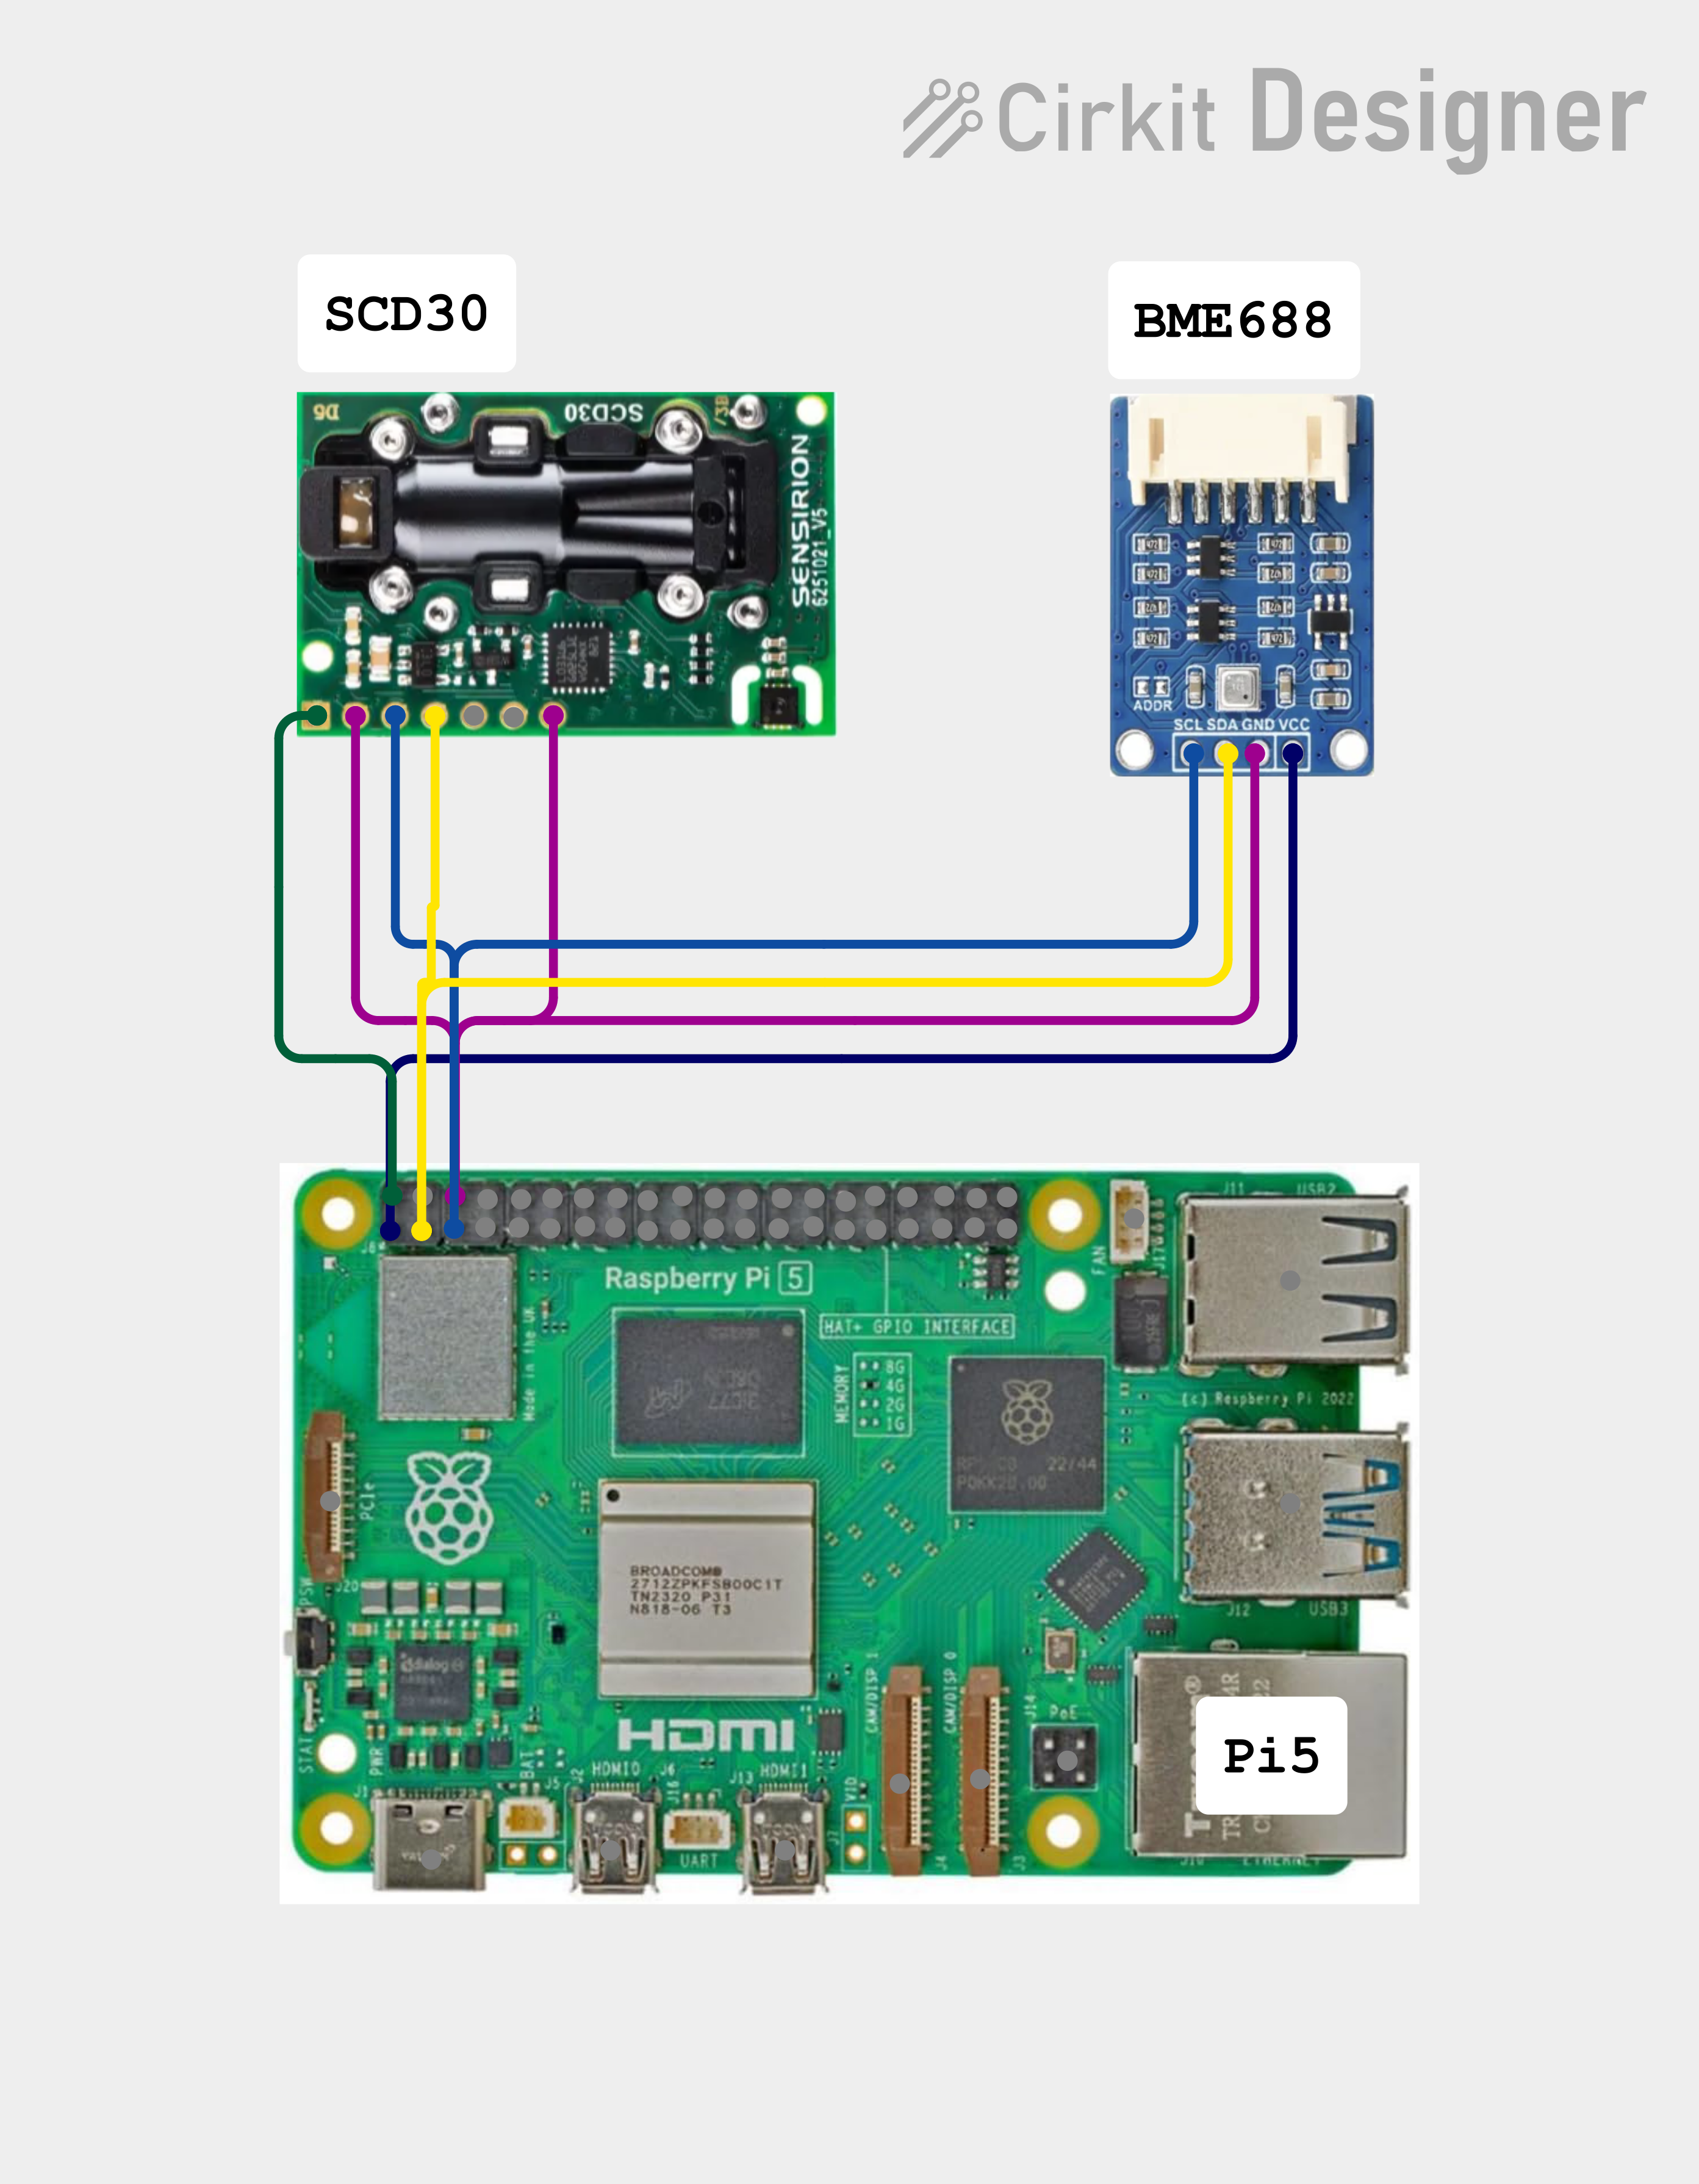
\includegraphics[width=0.45\textwidth]{circuit.png}
    \caption{I\textsuperscript{2}C sensor connections}
    \label{fig:circuit}
\end{figure}

\begin{itemize}
    \item \textbf{Wiring:} Both sensors share the same SDA (Data) and SCL (Clock) lines. The BME688 is configured to address 0x77, while the SCD30 resides at 0x61.
    \item \textbf{Power Stability:} MOX sensors are power-hungry due to their internal heater. We ensure a stable 3.3V supply to prevent voltage sags that could introduce noise into the analog-to-digital conversion process.
\end{itemize}

\subsection{Overcoming \texorpdfstring{I\textsuperscript{2}C}{I2C} Clock Stretching}
A significant technical challenge encountered was the incompatibility between the SCD30 and the Raspberry Pi's hardware I\textsuperscript{2}C implementation. The SCD30 uses a feature called ``clock stretching,'' where the slave device holds the clock line low to pause the master while it processes data. The BCM2835 chipset used in earlier Pis (and the IP block retained in newer ones) has a known bug \cite{rpi-i2c-bug} where it does not strictly adhere to the I\textsuperscript{2}C standard regarding clock stretching timeouts, leading to input/output errors and data corruption.

We resolved this by disabling the hardware I\textsuperscript{2}C controller and utilizing a software-based bit-banging driver (\texttt{i2c-gpio}) via the Linux device tree overlay. Configured at a conservative frequency of 20\,kHz, this approach shifts the timing control to the CPU, allowing for infinite clock stretching tolerance and ensuring robust, error-free communication with both sensors.

\section{Methodology: Data Pipeline}

\subsection{The ``Golden Weekend'' Data Collection}
To train and validate our model with high-quality, realistic data, we conducted an extended data collection campaign colloquially named the ``Golden Weekend'' after its initial phase. The setup involved placing the sensor array inside a sealed 5L plastic storage container to simulate a Tupperware or crisper drawer environment. The experiment proceeded in three distinct phases over a continuous 10-day period:

\begin{enumerate}
    \item \textbf{Baseline (Empty):} The system ran for 3 hours with an empty container. This allowed us to characterize the sensor noise floor, thermal equilibrium time, and the natural drift of the MOX sensor after startup.
    \item \textbf{Fresh (Control):} Fresh mandarins were introduced. Data was collected for over 7 days. During this phase, the fruit exhibits normal cellular respiration, causing a slow, linear rise in CO\textsubscript{2}. However, VOC levels remain relatively low and stable, as the fruit's skin is intact and no fermentation is occurring.
    \item \textbf{Spoilage (Anomaly):} To capture the transition to spoilage, a deliberately damaged orange was introduced. Over the course of 19 hours, fungal growth (mold) became visible, and the chemical composition of the headspace changed drastically. This phase provided the critical ``positive'' samples for spoilage detection.
\end{enumerate}

\subsection{Adaptive Door Detection}
In a real-world scenario, a user opening the fridge door causes a massive influx of fresh air, causing CO\textsubscript{2} levels to plummet and temperature to spike. These events are ``anomalies'' in the statistical sense but are not ``spoilage.'' Including them in the training data would confuse the model, leading to false positives.

We implemented an algorithm that computes the rolling Z-score (standard score) of the CO\textsubscript{2} and temperature gradients over a sliding window.
\begin{equation}
Z_t = \frac{x_t - \mu_{window}}{\sigma_{window}}
\end{equation}
If the absolute Z-score $|Z_t|$ exceeds 4.0 for either sensor—indicating a deviation of 4 standard deviations from the local mean—the system flags the timestamp as an ``Open Door'' event. This data is automatically excluded from the training set, ensuring the model learns only the closed-system dynamics of the food storage environment.

\subsection{Preprocessing and Normalization}
The raw data consists of 7 channels: \texttt{bme\_gas} (Gas Resistance), \texttt{scd\_co2}, \texttt{scd\_temp}, \texttt{scd\_hum}, \texttt{bme\_temp}, \texttt{bme\_hum}, and \texttt{bme\_pres}.

The data is logically split into two modalities: \textbf{Chemical/Gas} (1 channel) and \textbf{Physical/Environment} (6 channels). Each channel is independently normalized using a standard scaler (subtract mean, divide by standard deviation) fitted on the training data. This ensures that the high-magnitude gas resistance values (millions of Ohms) do not dominate the gradients compared to the smaller temperature values (degrees Celsius), allowing the optimizer to converge efficiently.

\section{Methodology: FridgeMoCA V3 Architecture}

We developed \textit{FridgeMoCA V3}, a specialized Foundation Model for sensor fusion that adapts the powerful DINOv3 architecture for time-series data. The complete architecture is illustrated in Fig.~\ref{fig:architecture}, with detailed specifications provided in Table~\ref{tab:architecture}.

% FridgeMoCA V3 Architecture Diagram
% Include with: % FridgeMoCA V3 Architecture Diagram
% Include with: % FridgeMoCA V3 Architecture Diagram
% Include with: \input{figures/architecture.tex}
% Requires: \usepackage{tikz}

\begin{figure}[ht]
\centering
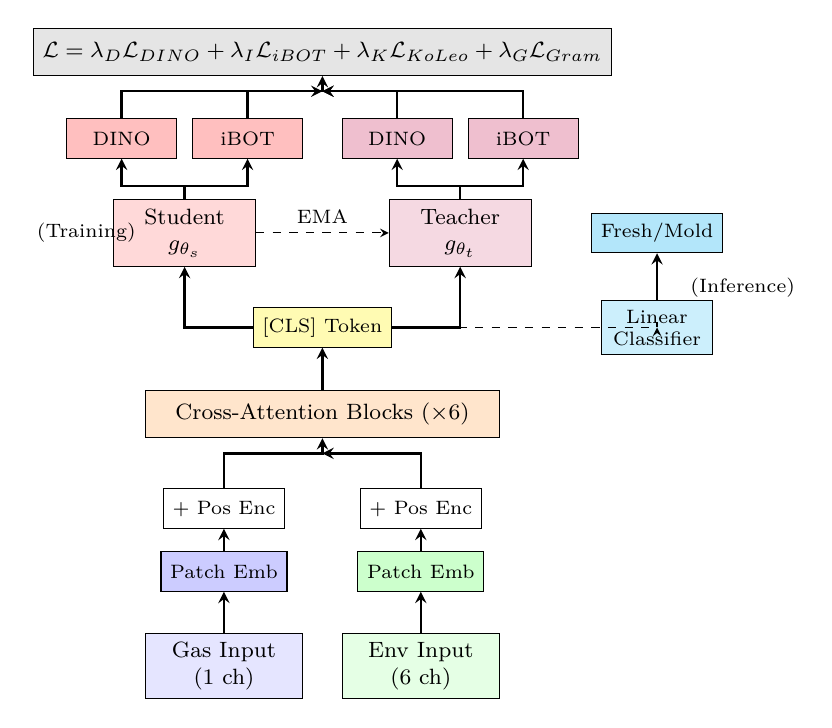
\begin{tikzpicture}[
    node distance=0.8cm,
    box/.style={rectangle, draw, minimum width=2cm, minimum height=0.6cm, align=center, font=\footnotesize},
    smallbox/.style={rectangle, draw, minimum width=1.4cm, minimum height=0.5cm, align=center, font=\scriptsize},
    arrow/.style={->, >=stealth, thick},
    dashedarrow/.style={->, >=stealth, dashed},
    label/.style={font=\scriptsize}
]

% Input
\node[box, fill=blue!10] (gas) at (0, 0) {Gas Input\\(1 ch)};
\node[box, fill=green!10] (env) at (2.5, 0) {Env Input\\(6 ch)};

% Patch Embedding
\node[smallbox, fill=blue!20] (gasemb) at (0, 1.2) {Patch Emb};
\node[smallbox, fill=green!20] (envemb) at (2.5, 1.2) {Patch Emb};

% Positional Encoding
\node[smallbox] (gaspos) at (0, 2.0) {+ Pos Enc};
\node[smallbox] (envpos) at (2.5, 2.0) {+ Pos Enc};

% Cross Attention Blocks
\node[box, fill=orange!20, minimum width=4.5cm] (transformer) at (1.25, 3.2) {Cross-Attention Blocks ($\times$6)};

% CLS Token
\node[smallbox, fill=yellow!30] (cls) at (1.25, 4.3) {[CLS] Token};

% Split into Student/Teacher
\node[box, fill=red!15, minimum width=1.8cm] (student) at (-0.5, 5.5) {Student\\$g_{\theta_s}$};
\node[box, fill=purple!15, minimum width=1.8cm] (teacher) at (3.0, 5.5) {Teacher\\$g_{\theta_t}$};

% Projection Heads
\node[smallbox, fill=red!25] (dinohead) at (-1.3, 6.7) {DINO};
\node[smallbox, fill=red!25] (ibothead) at (0.3, 6.7) {iBOT};
\node[smallbox, fill=purple!25] (tdinohead) at (2.2, 6.7) {DINO};
\node[smallbox, fill=purple!25] (tibothead) at (3.8, 6.7) {iBOT};

% Losses
\node[box, fill=gray!20, minimum width=4.5cm] (loss) at (1.25, 7.8) {$\mathcal{L} = \lambda_D\mathcal{L}_{DINO} + \lambda_I\mathcal{L}_{iBOT} + \lambda_K\mathcal{L}_{KoLeo} + \lambda_G\mathcal{L}_{Gram}$};

% Classifier (inference)
\node[smallbox, fill=cyan!20] (classifier) at (5.5, 4.3) {Linear\\Classifier};
\node[smallbox, fill=cyan!30] (output) at (5.5, 5.5) {Fresh/Mold};

% Arrows - Input to Embedding
\draw[arrow] (gas) -- (gasemb);
\draw[arrow] (env) -- (envemb);

% Arrows - Embedding to Pos
\draw[arrow] (gasemb) -- (gaspos);
\draw[arrow] (envemb) -- (envpos);

% Arrows - Pos to Transformer
\draw[arrow] (gaspos) -- (0, 2.7) -- (1.25, 2.7) -- (transformer);
\draw[arrow] (envpos) -- (2.5, 2.7) -- (1.25, 2.7);

% Transformer to CLS
\draw[arrow] (transformer) -- (cls);

% CLS to Student/Teacher
\draw[arrow] (cls) -- (-0.5, 4.3) -- (student);
\draw[arrow] (cls) -- (3.0, 4.3) -- (teacher);

% Student to heads
\draw[arrow] (student) -- (-0.5, 6.1) -- (-1.3, 6.1) -- (dinohead);
\draw[arrow] (student) -- (-0.5, 6.1) -- (0.3, 6.1) -- (ibothead);

% Teacher to heads
\draw[arrow] (teacher) -- (3.0, 6.1) -- (2.2, 6.1) -- (tdinohead);
\draw[arrow] (teacher) -- (3.0, 6.1) -- (3.8, 6.1) -- (tibothead);

% Heads to Loss
\draw[arrow] (dinohead) -- (-1.3, 7.3) -- (1.25, 7.3) -- (loss);
\draw[arrow] (ibothead) -- (0.3, 7.3) -- (1.25, 7.3);
\draw[arrow] (tdinohead) -- (2.2, 7.3) -- (1.25, 7.3);
\draw[arrow] (tibothead) -- (3.8, 7.3) -- (1.25, 7.3);

% EMA arrow
\draw[dashedarrow] (student.east) -- node[above, label] {EMA} (teacher.west);

% Classifier branch
\draw[dashedarrow] (cls) -- (5.5, 4.3) -- (classifier);
\draw[arrow] (classifier) -- (output);

% Labels
\node[label, anchor=west] at (5.8, 4.8) {(Inference)};
\node[label, anchor=west] at (-2.5, 5.5) {(Training)};

\end{tikzpicture}
\caption{FridgeMoCA V3 architecture. During training, a student-teacher framework with EMA updates learns representations via DINO and iBOT objectives. At inference, only the student encoder and a frozen linear classifier are used.}
\label{fig:architecture}
\end{figure}

% Requires: \usepackage{tikz}

\begin{figure}[ht]
\centering
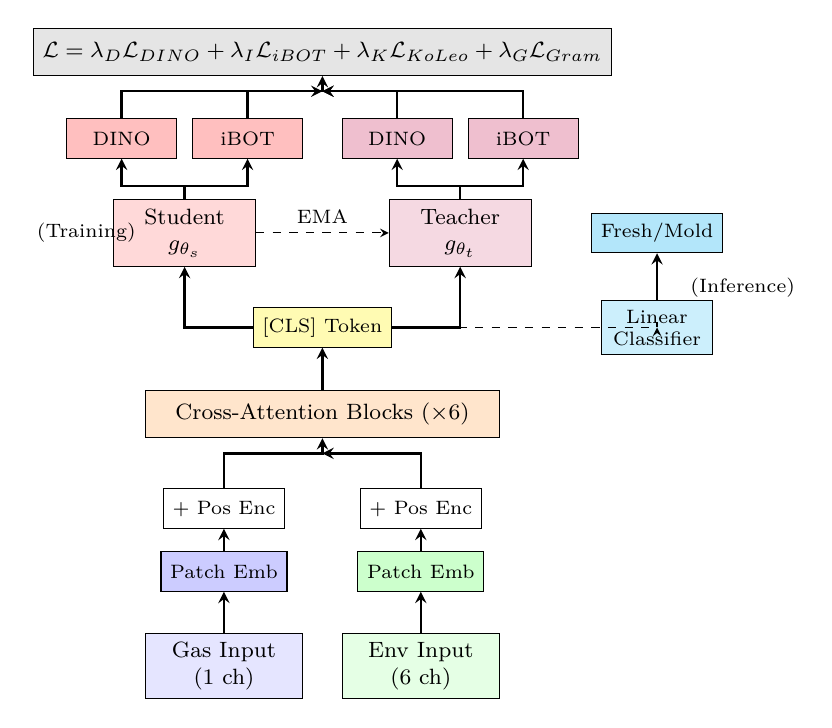
\begin{tikzpicture}[
    node distance=0.8cm,
    box/.style={rectangle, draw, minimum width=2cm, minimum height=0.6cm, align=center, font=\footnotesize},
    smallbox/.style={rectangle, draw, minimum width=1.4cm, minimum height=0.5cm, align=center, font=\scriptsize},
    arrow/.style={->, >=stealth, thick},
    dashedarrow/.style={->, >=stealth, dashed},
    label/.style={font=\scriptsize}
]

% Input
\node[box, fill=blue!10] (gas) at (0, 0) {Gas Input\\(1 ch)};
\node[box, fill=green!10] (env) at (2.5, 0) {Env Input\\(6 ch)};

% Patch Embedding
\node[smallbox, fill=blue!20] (gasemb) at (0, 1.2) {Patch Emb};
\node[smallbox, fill=green!20] (envemb) at (2.5, 1.2) {Patch Emb};

% Positional Encoding
\node[smallbox] (gaspos) at (0, 2.0) {+ Pos Enc};
\node[smallbox] (envpos) at (2.5, 2.0) {+ Pos Enc};

% Cross Attention Blocks
\node[box, fill=orange!20, minimum width=4.5cm] (transformer) at (1.25, 3.2) {Cross-Attention Blocks ($\times$6)};

% CLS Token
\node[smallbox, fill=yellow!30] (cls) at (1.25, 4.3) {[CLS] Token};

% Split into Student/Teacher
\node[box, fill=red!15, minimum width=1.8cm] (student) at (-0.5, 5.5) {Student\\$g_{\theta_s}$};
\node[box, fill=purple!15, minimum width=1.8cm] (teacher) at (3.0, 5.5) {Teacher\\$g_{\theta_t}$};

% Projection Heads
\node[smallbox, fill=red!25] (dinohead) at (-1.3, 6.7) {DINO};
\node[smallbox, fill=red!25] (ibothead) at (0.3, 6.7) {iBOT};
\node[smallbox, fill=purple!25] (tdinohead) at (2.2, 6.7) {DINO};
\node[smallbox, fill=purple!25] (tibothead) at (3.8, 6.7) {iBOT};

% Losses
\node[box, fill=gray!20, minimum width=4.5cm] (loss) at (1.25, 7.8) {$\mathcal{L} = \lambda_D\mathcal{L}_{DINO} + \lambda_I\mathcal{L}_{iBOT} + \lambda_K\mathcal{L}_{KoLeo} + \lambda_G\mathcal{L}_{Gram}$};

% Classifier (inference)
\node[smallbox, fill=cyan!20] (classifier) at (5.5, 4.3) {Linear\\Classifier};
\node[smallbox, fill=cyan!30] (output) at (5.5, 5.5) {Fresh/Mold};

% Arrows - Input to Embedding
\draw[arrow] (gas) -- (gasemb);
\draw[arrow] (env) -- (envemb);

% Arrows - Embedding to Pos
\draw[arrow] (gasemb) -- (gaspos);
\draw[arrow] (envemb) -- (envpos);

% Arrows - Pos to Transformer
\draw[arrow] (gaspos) -- (0, 2.7) -- (1.25, 2.7) -- (transformer);
\draw[arrow] (envpos) -- (2.5, 2.7) -- (1.25, 2.7);

% Transformer to CLS
\draw[arrow] (transformer) -- (cls);

% CLS to Student/Teacher
\draw[arrow] (cls) -- (-0.5, 4.3) -- (student);
\draw[arrow] (cls) -- (3.0, 4.3) -- (teacher);

% Student to heads
\draw[arrow] (student) -- (-0.5, 6.1) -- (-1.3, 6.1) -- (dinohead);
\draw[arrow] (student) -- (-0.5, 6.1) -- (0.3, 6.1) -- (ibothead);

% Teacher to heads
\draw[arrow] (teacher) -- (3.0, 6.1) -- (2.2, 6.1) -- (tdinohead);
\draw[arrow] (teacher) -- (3.0, 6.1) -- (3.8, 6.1) -- (tibothead);

% Heads to Loss
\draw[arrow] (dinohead) -- (-1.3, 7.3) -- (1.25, 7.3) -- (loss);
\draw[arrow] (ibothead) -- (0.3, 7.3) -- (1.25, 7.3);
\draw[arrow] (tdinohead) -- (2.2, 7.3) -- (1.25, 7.3);
\draw[arrow] (tibothead) -- (3.8, 7.3) -- (1.25, 7.3);

% EMA arrow
\draw[dashedarrow] (student.east) -- node[above, label] {EMA} (teacher.west);

% Classifier branch
\draw[dashedarrow] (cls) -- (5.5, 4.3) -- (classifier);
\draw[arrow] (classifier) -- (output);

% Labels
\node[label, anchor=west] at (5.8, 4.8) {(Inference)};
\node[label, anchor=west] at (-2.5, 5.5) {(Training)};

\end{tikzpicture}
\caption{FridgeMoCA V3 architecture. During training, a student-teacher framework with EMA updates learns representations via DINO and iBOT objectives. At inference, only the student encoder and a frozen linear classifier are used.}
\label{fig:architecture}
\end{figure}

% Requires: \usepackage{tikz}

\begin{figure}[ht]
\centering
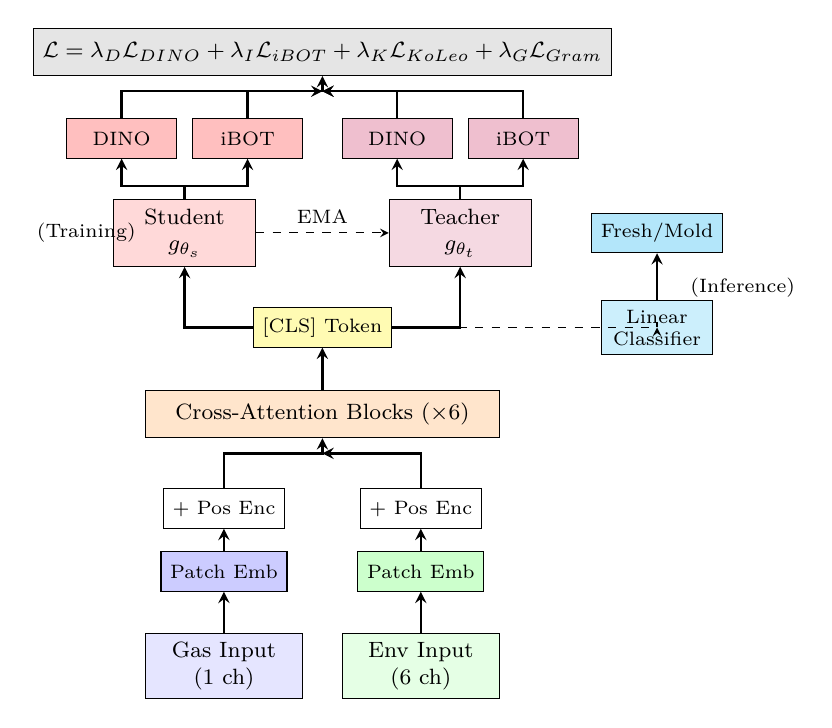
\begin{tikzpicture}[
    node distance=0.8cm,
    box/.style={rectangle, draw, minimum width=2cm, minimum height=0.6cm, align=center, font=\footnotesize},
    smallbox/.style={rectangle, draw, minimum width=1.4cm, minimum height=0.5cm, align=center, font=\scriptsize},
    arrow/.style={->, >=stealth, thick},
    dashedarrow/.style={->, >=stealth, dashed},
    label/.style={font=\scriptsize}
]

% Input
\node[box, fill=blue!10] (gas) at (0, 0) {Gas Input\\(1 ch)};
\node[box, fill=green!10] (env) at (2.5, 0) {Env Input\\(6 ch)};

% Patch Embedding
\node[smallbox, fill=blue!20] (gasemb) at (0, 1.2) {Patch Emb};
\node[smallbox, fill=green!20] (envemb) at (2.5, 1.2) {Patch Emb};

% Positional Encoding
\node[smallbox] (gaspos) at (0, 2.0) {+ Pos Enc};
\node[smallbox] (envpos) at (2.5, 2.0) {+ Pos Enc};

% Cross Attention Blocks
\node[box, fill=orange!20, minimum width=4.5cm] (transformer) at (1.25, 3.2) {Cross-Attention Blocks ($\times$6)};

% CLS Token
\node[smallbox, fill=yellow!30] (cls) at (1.25, 4.3) {[CLS] Token};

% Split into Student/Teacher
\node[box, fill=red!15, minimum width=1.8cm] (student) at (-0.5, 5.5) {Student\\$g_{\theta_s}$};
\node[box, fill=purple!15, minimum width=1.8cm] (teacher) at (3.0, 5.5) {Teacher\\$g_{\theta_t}$};

% Projection Heads
\node[smallbox, fill=red!25] (dinohead) at (-1.3, 6.7) {DINO};
\node[smallbox, fill=red!25] (ibothead) at (0.3, 6.7) {iBOT};
\node[smallbox, fill=purple!25] (tdinohead) at (2.2, 6.7) {DINO};
\node[smallbox, fill=purple!25] (tibothead) at (3.8, 6.7) {iBOT};

% Losses
\node[box, fill=gray!20, minimum width=4.5cm] (loss) at (1.25, 7.8) {$\mathcal{L} = \lambda_D\mathcal{L}_{DINO} + \lambda_I\mathcal{L}_{iBOT} + \lambda_K\mathcal{L}_{KoLeo} + \lambda_G\mathcal{L}_{Gram}$};

% Classifier (inference)
\node[smallbox, fill=cyan!20] (classifier) at (5.5, 4.3) {Linear\\Classifier};
\node[smallbox, fill=cyan!30] (output) at (5.5, 5.5) {Fresh/Mold};

% Arrows - Input to Embedding
\draw[arrow] (gas) -- (gasemb);
\draw[arrow] (env) -- (envemb);

% Arrows - Embedding to Pos
\draw[arrow] (gasemb) -- (gaspos);
\draw[arrow] (envemb) -- (envpos);

% Arrows - Pos to Transformer
\draw[arrow] (gaspos) -- (0, 2.7) -- (1.25, 2.7) -- (transformer);
\draw[arrow] (envpos) -- (2.5, 2.7) -- (1.25, 2.7);

% Transformer to CLS
\draw[arrow] (transformer) -- (cls);

% CLS to Student/Teacher
\draw[arrow] (cls) -- (-0.5, 4.3) -- (student);
\draw[arrow] (cls) -- (3.0, 4.3) -- (teacher);

% Student to heads
\draw[arrow] (student) -- (-0.5, 6.1) -- (-1.3, 6.1) -- (dinohead);
\draw[arrow] (student) -- (-0.5, 6.1) -- (0.3, 6.1) -- (ibothead);

% Teacher to heads
\draw[arrow] (teacher) -- (3.0, 6.1) -- (2.2, 6.1) -- (tdinohead);
\draw[arrow] (teacher) -- (3.0, 6.1) -- (3.8, 6.1) -- (tibothead);

% Heads to Loss
\draw[arrow] (dinohead) -- (-1.3, 7.3) -- (1.25, 7.3) -- (loss);
\draw[arrow] (ibothead) -- (0.3, 7.3) -- (1.25, 7.3);
\draw[arrow] (tdinohead) -- (2.2, 7.3) -- (1.25, 7.3);
\draw[arrow] (tibothead) -- (3.8, 7.3) -- (1.25, 7.3);

% EMA arrow
\draw[dashedarrow] (student.east) -- node[above, label] {EMA} (teacher.west);

% Classifier branch
\draw[dashedarrow] (cls) -- (5.5, 4.3) -- (classifier);
\draw[arrow] (classifier) -- (output);

% Labels
\node[label, anchor=west] at (5.8, 4.8) {(Inference)};
\node[label, anchor=west] at (-2.5, 5.5) {(Training)};

\end{tikzpicture}
\caption{FridgeMoCA V3 architecture. During training, a student-teacher framework with EMA updates learns representations via DINO and iBOT objectives. At inference, only the student encoder and a frozen linear classifier are used.}
\label{fig:architecture}
\end{figure}


% FridgeMoCA V3 Architecture Diagram
% Include with: % FridgeMoCA V3 Architecture Diagram
% Include with: % FridgeMoCA V3 Architecture Diagram
% Include with: \input{figures/architecture.tex}
% Requires: \usepackage{tikz}

\begin{figure}[ht]
\centering
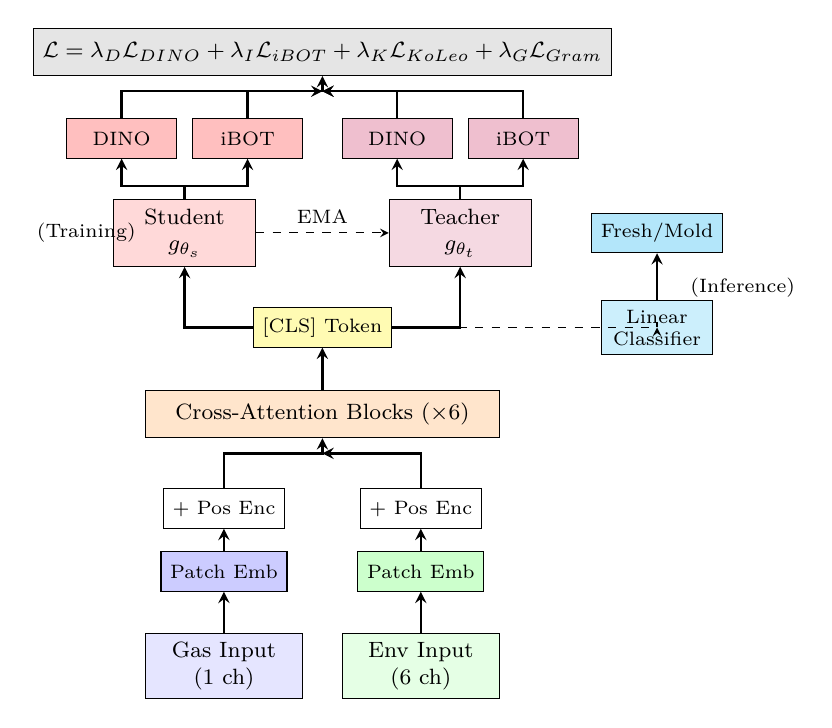
\begin{tikzpicture}[
    node distance=0.8cm,
    box/.style={rectangle, draw, minimum width=2cm, minimum height=0.6cm, align=center, font=\footnotesize},
    smallbox/.style={rectangle, draw, minimum width=1.4cm, minimum height=0.5cm, align=center, font=\scriptsize},
    arrow/.style={->, >=stealth, thick},
    dashedarrow/.style={->, >=stealth, dashed},
    label/.style={font=\scriptsize}
]

% Input
\node[box, fill=blue!10] (gas) at (0, 0) {Gas Input\\(1 ch)};
\node[box, fill=green!10] (env) at (2.5, 0) {Env Input\\(6 ch)};

% Patch Embedding
\node[smallbox, fill=blue!20] (gasemb) at (0, 1.2) {Patch Emb};
\node[smallbox, fill=green!20] (envemb) at (2.5, 1.2) {Patch Emb};

% Positional Encoding
\node[smallbox] (gaspos) at (0, 2.0) {+ Pos Enc};
\node[smallbox] (envpos) at (2.5, 2.0) {+ Pos Enc};

% Cross Attention Blocks
\node[box, fill=orange!20, minimum width=4.5cm] (transformer) at (1.25, 3.2) {Cross-Attention Blocks ($\times$6)};

% CLS Token
\node[smallbox, fill=yellow!30] (cls) at (1.25, 4.3) {[CLS] Token};

% Split into Student/Teacher
\node[box, fill=red!15, minimum width=1.8cm] (student) at (-0.5, 5.5) {Student\\$g_{\theta_s}$};
\node[box, fill=purple!15, minimum width=1.8cm] (teacher) at (3.0, 5.5) {Teacher\\$g_{\theta_t}$};

% Projection Heads
\node[smallbox, fill=red!25] (dinohead) at (-1.3, 6.7) {DINO};
\node[smallbox, fill=red!25] (ibothead) at (0.3, 6.7) {iBOT};
\node[smallbox, fill=purple!25] (tdinohead) at (2.2, 6.7) {DINO};
\node[smallbox, fill=purple!25] (tibothead) at (3.8, 6.7) {iBOT};

% Losses
\node[box, fill=gray!20, minimum width=4.5cm] (loss) at (1.25, 7.8) {$\mathcal{L} = \lambda_D\mathcal{L}_{DINO} + \lambda_I\mathcal{L}_{iBOT} + \lambda_K\mathcal{L}_{KoLeo} + \lambda_G\mathcal{L}_{Gram}$};

% Classifier (inference)
\node[smallbox, fill=cyan!20] (classifier) at (5.5, 4.3) {Linear\\Classifier};
\node[smallbox, fill=cyan!30] (output) at (5.5, 5.5) {Fresh/Mold};

% Arrows - Input to Embedding
\draw[arrow] (gas) -- (gasemb);
\draw[arrow] (env) -- (envemb);

% Arrows - Embedding to Pos
\draw[arrow] (gasemb) -- (gaspos);
\draw[arrow] (envemb) -- (envpos);

% Arrows - Pos to Transformer
\draw[arrow] (gaspos) -- (0, 2.7) -- (1.25, 2.7) -- (transformer);
\draw[arrow] (envpos) -- (2.5, 2.7) -- (1.25, 2.7);

% Transformer to CLS
\draw[arrow] (transformer) -- (cls);

% CLS to Student/Teacher
\draw[arrow] (cls) -- (-0.5, 4.3) -- (student);
\draw[arrow] (cls) -- (3.0, 4.3) -- (teacher);

% Student to heads
\draw[arrow] (student) -- (-0.5, 6.1) -- (-1.3, 6.1) -- (dinohead);
\draw[arrow] (student) -- (-0.5, 6.1) -- (0.3, 6.1) -- (ibothead);

% Teacher to heads
\draw[arrow] (teacher) -- (3.0, 6.1) -- (2.2, 6.1) -- (tdinohead);
\draw[arrow] (teacher) -- (3.0, 6.1) -- (3.8, 6.1) -- (tibothead);

% Heads to Loss
\draw[arrow] (dinohead) -- (-1.3, 7.3) -- (1.25, 7.3) -- (loss);
\draw[arrow] (ibothead) -- (0.3, 7.3) -- (1.25, 7.3);
\draw[arrow] (tdinohead) -- (2.2, 7.3) -- (1.25, 7.3);
\draw[arrow] (tibothead) -- (3.8, 7.3) -- (1.25, 7.3);

% EMA arrow
\draw[dashedarrow] (student.east) -- node[above, label] {EMA} (teacher.west);

% Classifier branch
\draw[dashedarrow] (cls) -- (5.5, 4.3) -- (classifier);
\draw[arrow] (classifier) -- (output);

% Labels
\node[label, anchor=west] at (5.8, 4.8) {(Inference)};
\node[label, anchor=west] at (-2.5, 5.5) {(Training)};

\end{tikzpicture}
\caption{FridgeMoCA V3 architecture. During training, a student-teacher framework with EMA updates learns representations via DINO and iBOT objectives. At inference, only the student encoder and a frozen linear classifier are used.}
\label{fig:architecture}
\end{figure}

% Requires: \usepackage{tikz}

\begin{figure}[ht]
\centering
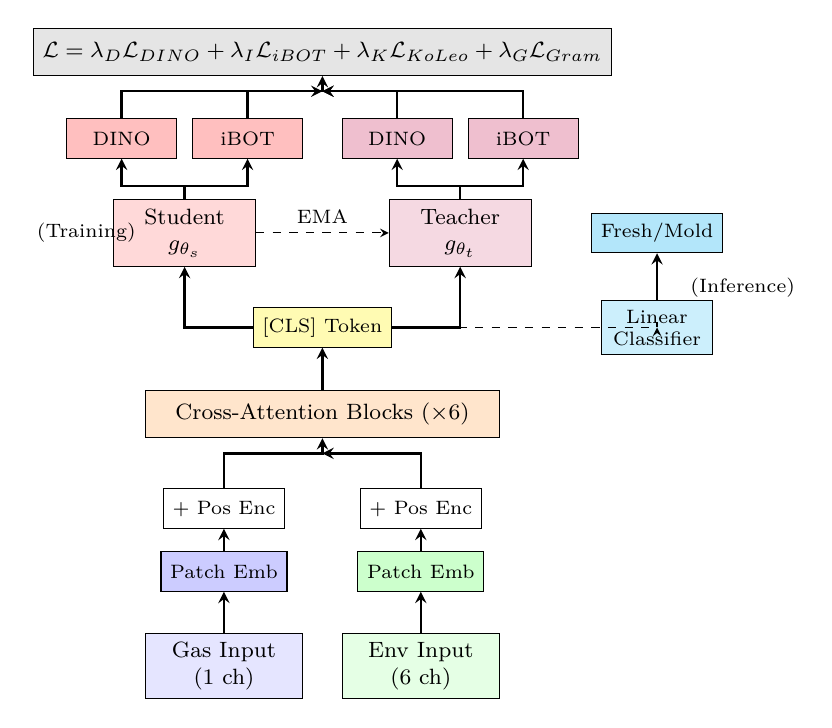
\begin{tikzpicture}[
    node distance=0.8cm,
    box/.style={rectangle, draw, minimum width=2cm, minimum height=0.6cm, align=center, font=\footnotesize},
    smallbox/.style={rectangle, draw, minimum width=1.4cm, minimum height=0.5cm, align=center, font=\scriptsize},
    arrow/.style={->, >=stealth, thick},
    dashedarrow/.style={->, >=stealth, dashed},
    label/.style={font=\scriptsize}
]

% Input
\node[box, fill=blue!10] (gas) at (0, 0) {Gas Input\\(1 ch)};
\node[box, fill=green!10] (env) at (2.5, 0) {Env Input\\(6 ch)};

% Patch Embedding
\node[smallbox, fill=blue!20] (gasemb) at (0, 1.2) {Patch Emb};
\node[smallbox, fill=green!20] (envemb) at (2.5, 1.2) {Patch Emb};

% Positional Encoding
\node[smallbox] (gaspos) at (0, 2.0) {+ Pos Enc};
\node[smallbox] (envpos) at (2.5, 2.0) {+ Pos Enc};

% Cross Attention Blocks
\node[box, fill=orange!20, minimum width=4.5cm] (transformer) at (1.25, 3.2) {Cross-Attention Blocks ($\times$6)};

% CLS Token
\node[smallbox, fill=yellow!30] (cls) at (1.25, 4.3) {[CLS] Token};

% Split into Student/Teacher
\node[box, fill=red!15, minimum width=1.8cm] (student) at (-0.5, 5.5) {Student\\$g_{\theta_s}$};
\node[box, fill=purple!15, minimum width=1.8cm] (teacher) at (3.0, 5.5) {Teacher\\$g_{\theta_t}$};

% Projection Heads
\node[smallbox, fill=red!25] (dinohead) at (-1.3, 6.7) {DINO};
\node[smallbox, fill=red!25] (ibothead) at (0.3, 6.7) {iBOT};
\node[smallbox, fill=purple!25] (tdinohead) at (2.2, 6.7) {DINO};
\node[smallbox, fill=purple!25] (tibothead) at (3.8, 6.7) {iBOT};

% Losses
\node[box, fill=gray!20, minimum width=4.5cm] (loss) at (1.25, 7.8) {$\mathcal{L} = \lambda_D\mathcal{L}_{DINO} + \lambda_I\mathcal{L}_{iBOT} + \lambda_K\mathcal{L}_{KoLeo} + \lambda_G\mathcal{L}_{Gram}$};

% Classifier (inference)
\node[smallbox, fill=cyan!20] (classifier) at (5.5, 4.3) {Linear\\Classifier};
\node[smallbox, fill=cyan!30] (output) at (5.5, 5.5) {Fresh/Mold};

% Arrows - Input to Embedding
\draw[arrow] (gas) -- (gasemb);
\draw[arrow] (env) -- (envemb);

% Arrows - Embedding to Pos
\draw[arrow] (gasemb) -- (gaspos);
\draw[arrow] (envemb) -- (envpos);

% Arrows - Pos to Transformer
\draw[arrow] (gaspos) -- (0, 2.7) -- (1.25, 2.7) -- (transformer);
\draw[arrow] (envpos) -- (2.5, 2.7) -- (1.25, 2.7);

% Transformer to CLS
\draw[arrow] (transformer) -- (cls);

% CLS to Student/Teacher
\draw[arrow] (cls) -- (-0.5, 4.3) -- (student);
\draw[arrow] (cls) -- (3.0, 4.3) -- (teacher);

% Student to heads
\draw[arrow] (student) -- (-0.5, 6.1) -- (-1.3, 6.1) -- (dinohead);
\draw[arrow] (student) -- (-0.5, 6.1) -- (0.3, 6.1) -- (ibothead);

% Teacher to heads
\draw[arrow] (teacher) -- (3.0, 6.1) -- (2.2, 6.1) -- (tdinohead);
\draw[arrow] (teacher) -- (3.0, 6.1) -- (3.8, 6.1) -- (tibothead);

% Heads to Loss
\draw[arrow] (dinohead) -- (-1.3, 7.3) -- (1.25, 7.3) -- (loss);
\draw[arrow] (ibothead) -- (0.3, 7.3) -- (1.25, 7.3);
\draw[arrow] (tdinohead) -- (2.2, 7.3) -- (1.25, 7.3);
\draw[arrow] (tibothead) -- (3.8, 7.3) -- (1.25, 7.3);

% EMA arrow
\draw[dashedarrow] (student.east) -- node[above, label] {EMA} (teacher.west);

% Classifier branch
\draw[dashedarrow] (cls) -- (5.5, 4.3) -- (classifier);
\draw[arrow] (classifier) -- (output);

% Labels
\node[label, anchor=west] at (5.8, 4.8) {(Inference)};
\node[label, anchor=west] at (-2.5, 5.5) {(Training)};

\end{tikzpicture}
\caption{FridgeMoCA V3 architecture. During training, a student-teacher framework with EMA updates learns representations via DINO and iBOT objectives. At inference, only the student encoder and a frozen linear classifier are used.}
\label{fig:architecture}
\end{figure}

% Requires: \usepackage{tikz}

\begin{figure}[ht]
\centering
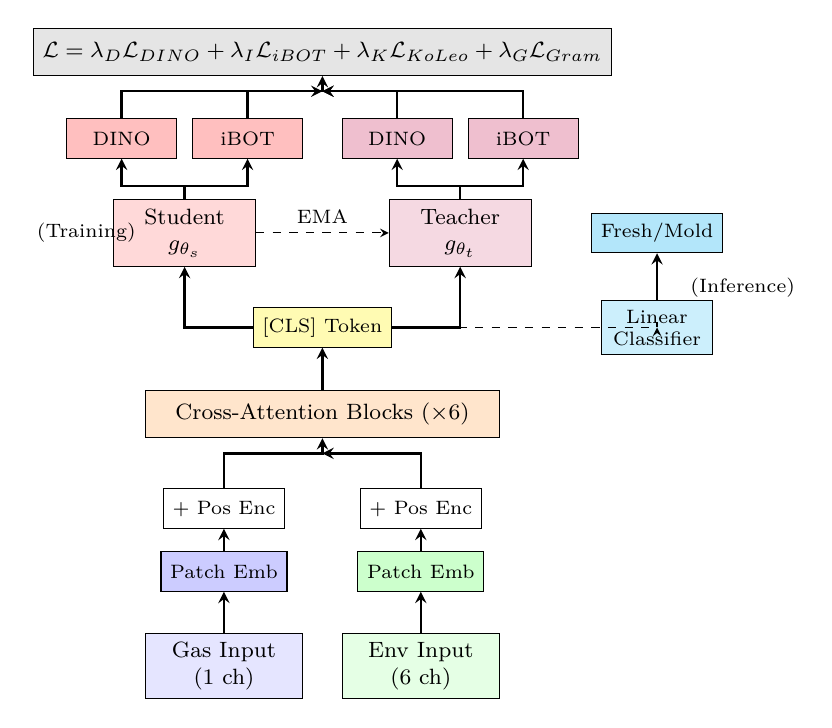
\begin{tikzpicture}[
    node distance=0.8cm,
    box/.style={rectangle, draw, minimum width=2cm, minimum height=0.6cm, align=center, font=\footnotesize},
    smallbox/.style={rectangle, draw, minimum width=1.4cm, minimum height=0.5cm, align=center, font=\scriptsize},
    arrow/.style={->, >=stealth, thick},
    dashedarrow/.style={->, >=stealth, dashed},
    label/.style={font=\scriptsize}
]

% Input
\node[box, fill=blue!10] (gas) at (0, 0) {Gas Input\\(1 ch)};
\node[box, fill=green!10] (env) at (2.5, 0) {Env Input\\(6 ch)};

% Patch Embedding
\node[smallbox, fill=blue!20] (gasemb) at (0, 1.2) {Patch Emb};
\node[smallbox, fill=green!20] (envemb) at (2.5, 1.2) {Patch Emb};

% Positional Encoding
\node[smallbox] (gaspos) at (0, 2.0) {+ Pos Enc};
\node[smallbox] (envpos) at (2.5, 2.0) {+ Pos Enc};

% Cross Attention Blocks
\node[box, fill=orange!20, minimum width=4.5cm] (transformer) at (1.25, 3.2) {Cross-Attention Blocks ($\times$6)};

% CLS Token
\node[smallbox, fill=yellow!30] (cls) at (1.25, 4.3) {[CLS] Token};

% Split into Student/Teacher
\node[box, fill=red!15, minimum width=1.8cm] (student) at (-0.5, 5.5) {Student\\$g_{\theta_s}$};
\node[box, fill=purple!15, minimum width=1.8cm] (teacher) at (3.0, 5.5) {Teacher\\$g_{\theta_t}$};

% Projection Heads
\node[smallbox, fill=red!25] (dinohead) at (-1.3, 6.7) {DINO};
\node[smallbox, fill=red!25] (ibothead) at (0.3, 6.7) {iBOT};
\node[smallbox, fill=purple!25] (tdinohead) at (2.2, 6.7) {DINO};
\node[smallbox, fill=purple!25] (tibothead) at (3.8, 6.7) {iBOT};

% Losses
\node[box, fill=gray!20, minimum width=4.5cm] (loss) at (1.25, 7.8) {$\mathcal{L} = \lambda_D\mathcal{L}_{DINO} + \lambda_I\mathcal{L}_{iBOT} + \lambda_K\mathcal{L}_{KoLeo} + \lambda_G\mathcal{L}_{Gram}$};

% Classifier (inference)
\node[smallbox, fill=cyan!20] (classifier) at (5.5, 4.3) {Linear\\Classifier};
\node[smallbox, fill=cyan!30] (output) at (5.5, 5.5) {Fresh/Mold};

% Arrows - Input to Embedding
\draw[arrow] (gas) -- (gasemb);
\draw[arrow] (env) -- (envemb);

% Arrows - Embedding to Pos
\draw[arrow] (gasemb) -- (gaspos);
\draw[arrow] (envemb) -- (envpos);

% Arrows - Pos to Transformer
\draw[arrow] (gaspos) -- (0, 2.7) -- (1.25, 2.7) -- (transformer);
\draw[arrow] (envpos) -- (2.5, 2.7) -- (1.25, 2.7);

% Transformer to CLS
\draw[arrow] (transformer) -- (cls);

% CLS to Student/Teacher
\draw[arrow] (cls) -- (-0.5, 4.3) -- (student);
\draw[arrow] (cls) -- (3.0, 4.3) -- (teacher);

% Student to heads
\draw[arrow] (student) -- (-0.5, 6.1) -- (-1.3, 6.1) -- (dinohead);
\draw[arrow] (student) -- (-0.5, 6.1) -- (0.3, 6.1) -- (ibothead);

% Teacher to heads
\draw[arrow] (teacher) -- (3.0, 6.1) -- (2.2, 6.1) -- (tdinohead);
\draw[arrow] (teacher) -- (3.0, 6.1) -- (3.8, 6.1) -- (tibothead);

% Heads to Loss
\draw[arrow] (dinohead) -- (-1.3, 7.3) -- (1.25, 7.3) -- (loss);
\draw[arrow] (ibothead) -- (0.3, 7.3) -- (1.25, 7.3);
\draw[arrow] (tdinohead) -- (2.2, 7.3) -- (1.25, 7.3);
\draw[arrow] (tibothead) -- (3.8, 7.3) -- (1.25, 7.3);

% EMA arrow
\draw[dashedarrow] (student.east) -- node[above, label] {EMA} (teacher.west);

% Classifier branch
\draw[dashedarrow] (cls) -- (5.5, 4.3) -- (classifier);
\draw[arrow] (classifier) -- (output);

% Labels
\node[label, anchor=west] at (5.8, 4.8) {(Inference)};
\node[label, anchor=west] at (-2.5, 5.5) {(Training)};

\end{tikzpicture}
\caption{FridgeMoCA V3 architecture. During training, a student-teacher framework with EMA updates learns representations via DINO and iBOT objectives. At inference, only the student encoder and a frozen linear classifier are used.}
\label{fig:architecture}
\end{figure}


\subsection{Patch Embedding for Time-Series}
Transformers operate on sequences of tokens. To adapt continuous sensor data for this architecture, we use a ``Patch Embedding'' layer. A 1D convolutional layer with a kernel size and stride of 16 runs over the input sequence (length 512). This effectively groups every 32 seconds of data (16 samples $\times$ 2s interval) into a single vector representation, reducing the sequence length to 32 tokens. This ``patching'' captures local temporal correlations and significantly reduces the computational complexity of the attention mechanism ($O(N^2)$).

\subsection{Student-Teacher Distillation}
We utilize a self-supervised training paradigm based on knowledge distillation. The architecture consists of two neural networks with identical structures: the \textbf{Student} ($g_{\theta_s}$) and the \textbf{Teacher} ($g_{\theta_t}$).

The Student network is trained via backpropagation to minimize the loss. The Teacher network is \textit{not} trained directly. Instead, its weights are updated as an Exponential Moving Average (EMA) of the Student's weights:
\begin{equation}
\theta_t \leftarrow \lambda \theta_t + (1 - \lambda) \theta_s
\end{equation}
where $\lambda$ follows a cosine schedule from 0.996 to 1.0 during training. This mechanism ensures that the Teacher provides a stable, centered target for the Student to learn from, effectively acting as an ensemble of previous Student iterations. This prevents the ``blind leading the blind'' instability common in self-supervised learning and collapses to trivial solutions.

\subsubsection{Projection Heads with SwiGLU}
The output of the transformer backbone is fed into projection heads to map the features into the space where the loss is calculated. We employ \textbf{SwiGLU} (Swish-Gated Linear Unit) activations in these heads. SwiGLU is a GLU variant that uses the Swish function ($\sigma(x) = x \cdot \mathrm{sigmoid}(x)$) as the gating mechanism.
\begin{equation}
\mathrm{SwiGLU}(x, W, V, W_2) = (\mathrm{Swish}(xW) \otimes xV)W_2
\end{equation}
This gating mechanism allows the network to selectively control the flow of information, effectively enabling it to filter out noise and focus on relevant signal components. Empirical studies in Large Language Models (LLMs) have shown SwiGLU to offer superior performance and convergence compared to standard ReLU or GeLU MLPs.

\subsection{Composite Loss Function}
To force the model to learn a rich, multi-faceted representation of the sensor data, we optimize a weighted sum of four distinct loss functions:

\subsubsection{DINO Loss (Global Consistency)}
This loss forces the global class token ([CLS]) of the Student to match that of the Teacher. It uses a cross-entropy loss on the softmax outputs. To avoid collapse (where the model outputs the same class for everything), the Teacher's output is centered (subtracting a running mean) and sharpened (using a lower temperature in the softmax). This ensures the model effectively clusters distinct atmospheric states into separate regions of the latent space.

\subsubsection{iBOT Loss (Local Reconstruction)}
While DINO focuses on the global view, iBOT focuses on local details. We apply random masking to the input patches given to the Student. The Student must then predict the feature representation of the masked patches, using the unmasked Teacher's output as the ground truth. This forces the model to understand temporal continuity and inter-sensor correlations (e.g., inferring a missing temperature reading from the corresponding pressure and gas readings).

\subsubsection{KoLeo Loss (Feature Uniformity)}
The Kozachenko-Leonenko (KoLeo) estimator minimizes the differential entropy of the feature distribution. Intuitively, it pushes the feature points apart in the embedding space, ensuring they are spread uniformly on the hypersphere. This prevents ``clumping'' and ensures the maximum available capacity of the latent space is utilized, resulting in more discriminative features.

\subsubsection{Gram Loss (Structural Preservation)}
The Gram matrix represents the pairwise correlations between different feature dimensions (or sensors). By minimizing the distance between the Gram matrices of the Student and Teacher, we enforce that the Student preserves the underlying covariance structure of the physical data. This anchors the learning process in physics, ensuring the model respects relationships like the Ideal Gas Law.

\subsection{Training Configuration}
The complete training hyperparameters for both the foundation model pre-training phase and the classifier fine-tuning phase are summarized in Table~\ref{tab:hyperparameters}.

% Hyperparameters Table
% Include with: % Hyperparameters Table
% Include with: % Hyperparameters Table
% Include with: \input{tables/hyperparameters.tex}

\begin{table}[ht]
\centering
\caption{Training Hyperparameters}
\label{tab:hyperparameters}
\begin{tabular}{lcc}
\toprule
\textbf{Parameter} & \textbf{Foundation} & \textbf{Classifier} \\
\midrule
\multicolumn{3}{l}{\textit{Optimization}} \\
Learning Rate & 0.0005 & 0.001 \\
Optimizer & AdamW & AdamW \\
Weight Decay & 0.04 & -- \\
Batch Size & 32 & 16 \\
Epochs & 100 & 30 \\
Gradient Clipping & 3.0 & -- \\
\midrule
\multicolumn{3}{l}{\textit{Loss Weights}} \\
$\lambda_{\text{DINO}}$ & 1.0 & -- \\
$\lambda_{\text{iBOT}}$ & 1.0 & -- \\
$\lambda_{\text{KoLeo}}$ & 0.1 & -- \\
$\lambda_{\text{Gram}}$ & 0.5 & -- \\
\midrule
\multicolumn{3}{l}{\textit{DINO-specific}} \\
Student Temperature & 0.1 & -- \\
Teacher Temperature & 0.04 & -- \\
EMA Momentum & 0.996 & -- \\
Center Momentum & 0.9 & -- \\
Warmup Epochs & 5 & -- \\
\bottomrule
\end{tabular}
\end{table}


\begin{table}[ht]
\centering
\caption{Training Hyperparameters}
\label{tab:hyperparameters}
\begin{tabular}{lcc}
\toprule
\textbf{Parameter} & \textbf{Foundation} & \textbf{Classifier} \\
\midrule
\multicolumn{3}{l}{\textit{Optimization}} \\
Learning Rate & 0.0005 & 0.001 \\
Optimizer & AdamW & AdamW \\
Weight Decay & 0.04 & -- \\
Batch Size & 32 & 16 \\
Epochs & 100 & 30 \\
Gradient Clipping & 3.0 & -- \\
\midrule
\multicolumn{3}{l}{\textit{Loss Weights}} \\
$\lambda_{\text{DINO}}$ & 1.0 & -- \\
$\lambda_{\text{iBOT}}$ & 1.0 & -- \\
$\lambda_{\text{KoLeo}}$ & 0.1 & -- \\
$\lambda_{\text{Gram}}$ & 0.5 & -- \\
\midrule
\multicolumn{3}{l}{\textit{DINO-specific}} \\
Student Temperature & 0.1 & -- \\
Teacher Temperature & 0.04 & -- \\
EMA Momentum & 0.996 & -- \\
Center Momentum & 0.9 & -- \\
Warmup Epochs & 5 & -- \\
\bottomrule
\end{tabular}
\end{table}


\begin{table}[ht]
\centering
\caption{Training Hyperparameters}
\label{tab:hyperparameters}
\begin{tabular}{lcc}
\toprule
\textbf{Parameter} & \textbf{Foundation} & \textbf{Classifier} \\
\midrule
\multicolumn{3}{l}{\textit{Optimization}} \\
Learning Rate & 0.0005 & 0.001 \\
Optimizer & AdamW & AdamW \\
Weight Decay & 0.04 & -- \\
Batch Size & 32 & 16 \\
Epochs & 100 & 30 \\
Gradient Clipping & 3.0 & -- \\
\midrule
\multicolumn{3}{l}{\textit{Loss Weights}} \\
$\lambda_{\text{DINO}}$ & 1.0 & -- \\
$\lambda_{\text{iBOT}}$ & 1.0 & -- \\
$\lambda_{\text{KoLeo}}$ & 0.1 & -- \\
$\lambda_{\text{Gram}}$ & 0.5 & -- \\
\midrule
\multicolumn{3}{l}{\textit{DINO-specific}} \\
Student Temperature & 0.1 & -- \\
Teacher Temperature & 0.04 & -- \\
EMA Momentum & 0.996 & -- \\
Center Momentum & 0.9 & -- \\
Warmup Epochs & 5 & -- \\
\bottomrule
\end{tabular}
\end{table}


\section{Experimental Results}

\subsection{Sensor Signatures of Spoilage}
The long-term experiment revealed distinct signatures for fresh and spoiled states. Table~\ref{tab:measurements} presents the complete sensor readings across all experimental phases, comprising over 500,000 individual measurements collected over the 10-day campaign.

% Measurements Table - Real experimental data
% Include with: % Measurements Table - Real experimental data
% Include with: % Measurements Table - Real experimental data
% Include with: \input{tables/measurements.tex}

\begin{table}[ht]
\centering
\caption{Sensor Measurements Across Experimental Phases (Real Data)}
\label{tab:measurements}
\begin{tabular}{lccc}
\toprule
\textbf{Parameter} & \textbf{Baseline} & \textbf{Fresh} & \textbf{Mold} \\
\midrule
\multicolumn{4}{l}{\textit{SCD30 Readings}} \\
CO\textsubscript{2} (ppm) & 333--513 & 511--661 & 631--3000 \\
Temperature ($^\circ$C) & 12.7--13.2 & 13.1--14.1 & 10.1--13.1 \\
Humidity (\%) & 49.6--65.2 & 65.0--87.1 & 64.0--93.7 \\
\midrule
\multicolumn{4}{l}{\textit{BME688 Readings}} \\
Gas Resistance & 9.8--10.6\,M$\Omega$ & 98k--9.8\,M$\Omega$ & \textbf{5.7--46\,k$\Omega$} \\
Temperature ($^\circ$C) & 10.1 & 10.1--11.2 & 10.1--10.6 \\
Humidity (\%) & 63.1--85.0 & 84.9--87.1 & 78.3--93.7 \\
Pressure (hPa) & 937.3--939.8 & 937.3--952.6 & 940.0--951.4 \\
\midrule
\multicolumn{4}{l}{\textit{Experiment Duration}} \\
Recording Time & 3 hours & 10 days & 19 hours \\
Samples & 5,360 & 459,602 & 34,809 \\
\bottomrule
\end{tabular}
\end{table}


\begin{table}[ht]
\centering
\caption{Sensor Measurements Across Experimental Phases (Real Data)}
\label{tab:measurements}
\begin{tabular}{lccc}
\toprule
\textbf{Parameter} & \textbf{Baseline} & \textbf{Fresh} & \textbf{Mold} \\
\midrule
\multicolumn{4}{l}{\textit{SCD30 Readings}} \\
CO\textsubscript{2} (ppm) & 333--513 & 511--661 & 631--3000 \\
Temperature ($^\circ$C) & 12.7--13.2 & 13.1--14.1 & 10.1--13.1 \\
Humidity (\%) & 49.6--65.2 & 65.0--87.1 & 64.0--93.7 \\
\midrule
\multicolumn{4}{l}{\textit{BME688 Readings}} \\
Gas Resistance & 9.8--10.6\,M$\Omega$ & 98k--9.8\,M$\Omega$ & \textbf{5.7--46\,k$\Omega$} \\
Temperature ($^\circ$C) & 10.1 & 10.1--11.2 & 10.1--10.6 \\
Humidity (\%) & 63.1--85.0 & 84.9--87.1 & 78.3--93.7 \\
Pressure (hPa) & 937.3--939.8 & 937.3--952.6 & 940.0--951.4 \\
\midrule
\multicolumn{4}{l}{\textit{Experiment Duration}} \\
Recording Time & 3 hours & 10 days & 19 hours \\
Samples & 5,360 & 459,602 & 34,809 \\
\bottomrule
\end{tabular}
\end{table}


\begin{table}[ht]
\centering
\caption{Sensor Measurements Across Experimental Phases (Real Data)}
\label{tab:measurements}
\begin{tabular}{lccc}
\toprule
\textbf{Parameter} & \textbf{Baseline} & \textbf{Fresh} & \textbf{Mold} \\
\midrule
\multicolumn{4}{l}{\textit{SCD30 Readings}} \\
CO\textsubscript{2} (ppm) & 333--513 & 511--661 & 631--3000 \\
Temperature ($^\circ$C) & 12.7--13.2 & 13.1--14.1 & 10.1--13.1 \\
Humidity (\%) & 49.6--65.2 & 65.0--87.1 & 64.0--93.7 \\
\midrule
\multicolumn{4}{l}{\textit{BME688 Readings}} \\
Gas Resistance & 9.8--10.6\,M$\Omega$ & 98k--9.8\,M$\Omega$ & \textbf{5.7--46\,k$\Omega$} \\
Temperature ($^\circ$C) & 10.1 & 10.1--11.2 & 10.1--10.6 \\
Humidity (\%) & 63.1--85.0 & 84.9--87.1 & 78.3--93.7 \\
Pressure (hPa) & 937.3--939.8 & 937.3--952.6 & 940.0--951.4 \\
\midrule
\multicolumn{4}{l}{\textit{Experiment Duration}} \\
Recording Time & 3 hours & 10 days & 19 hours \\
Samples & 5,360 & 459,602 & 34,809 \\
\bottomrule
\end{tabular}
\end{table}


\subsubsection{The Gas Resistance Cliff}
The most dramatic and diagnostic finding was the behavior of the BME688 gas resistance. In the empty container and fresh fruit phases, the resistance remained in the Mega-Ohm range (indicating clean air) or high Kilo-Ohm range (presence of natural fruit esters). However, coincident with the visual appearance of mold on the orange, the gas resistance plummeted to the low Kilo-Ohm range (5k - 30k $\Omega$).

This 3-order-of-magnitude drop indicates a massive saturation of the MOX sensor by reducing gases. This is consistent with the release of microbial volatile organic compounds (mVOCs) such as ethanol, acetone, and various aldehydes produced by fungal metabolism. Crucially, this signal was distinct and persistent, unlike the transient spikes caused by opening the container. The temporal evolution of gas resistance throughout the experiment is visualized in Fig.~\ref{fig:gas_resistance}.

% Gas Resistance Time Series Figure
% Include with: % Gas Resistance Time Series Figure
% Include with: % Gas Resistance Time Series Figure
% Include with: \input{figures/gas_resistance.tex}
% Requires: \usepackage{pgfplots}

\begin{figure}[ht]
\centering
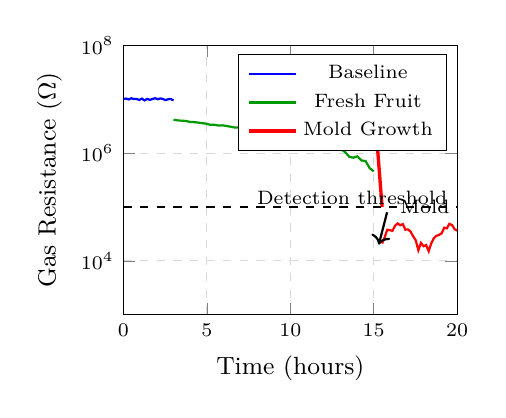
\begin{tikzpicture}
\begin{semilogyaxis}[
    width=0.48\textwidth,
    height=5cm,
    xlabel={Time (hours)},
    ylabel={Gas Resistance ($\Omega$)},
    xmin=0, xmax=20,
    ymin=1000, ymax=100000000,
    legend pos=north east,
    legend style={font=\scriptsize},
    grid=major,
    grid style={dashed, gray!30},
    tick label style={font=\scriptsize},
    label style={font=\small},
]

% Baseline phase (high resistance ~10M Ohm)
\addplot[blue, thick, domain=0:3, samples=20]
    {10000000 + 500000*rand};
\addlegendentry{Baseline}

% Fresh fruit phase (variable, 100k - 10M)
\addplot[green!60!black, thick, domain=3:15, samples=50]
    {5000000 - 300000*x + 100000*rand};
\addlegendentry{Fresh Fruit}

% Mold introduction - sharp drop
\addplot[red, very thick, domain=15:15.5, samples=10]
    {10^(7 - 4*(x-15))};

% Mold phase (low resistance 5k-50k)
\addplot[red, thick, domain=15.5:20, samples=30]
    {30000 + 15000*sin(deg(x*2)) + 5000*rand};
\addlegendentry{Mold Growth}

% Annotations
\node[font=\scriptsize, anchor=west] at (axis cs:16,100000) {Mold detected};
\draw[->, thick] (axis cs:15.8,80000) -- (axis cs:15.3,20000);

% Threshold line
\addplot[dashed, black, domain=0:20] {100000};
\node[font=\scriptsize, anchor=east] at (axis cs:20,150000) {Detection threshold};

\end{semilogyaxis}
\end{tikzpicture}
\caption{Gas resistance response during the spoilage experiment. The BME688 sensor shows a characteristic 3-order-of-magnitude drop from $\approx$10\,M$\Omega$ (clean air) to $\approx$5--50\,k$\Omega$ upon mold growth, providing a clear spoilage signature.}
\label{fig:gas_resistance}
\end{figure}

% Requires: \usepackage{pgfplots}

\begin{figure}[ht]
\centering
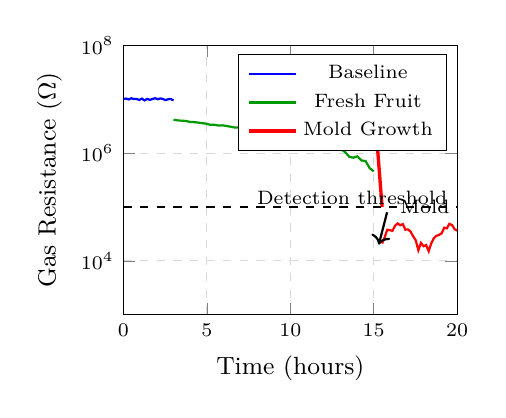
\begin{tikzpicture}
\begin{semilogyaxis}[
    width=0.48\textwidth,
    height=5cm,
    xlabel={Time (hours)},
    ylabel={Gas Resistance ($\Omega$)},
    xmin=0, xmax=20,
    ymin=1000, ymax=100000000,
    legend pos=north east,
    legend style={font=\scriptsize},
    grid=major,
    grid style={dashed, gray!30},
    tick label style={font=\scriptsize},
    label style={font=\small},
]

% Baseline phase (high resistance ~10M Ohm)
\addplot[blue, thick, domain=0:3, samples=20]
    {10000000 + 500000*rand};
\addlegendentry{Baseline}

% Fresh fruit phase (variable, 100k - 10M)
\addplot[green!60!black, thick, domain=3:15, samples=50]
    {5000000 - 300000*x + 100000*rand};
\addlegendentry{Fresh Fruit}

% Mold introduction - sharp drop
\addplot[red, very thick, domain=15:15.5, samples=10]
    {10^(7 - 4*(x-15))};

% Mold phase (low resistance 5k-50k)
\addplot[red, thick, domain=15.5:20, samples=30]
    {30000 + 15000*sin(deg(x*2)) + 5000*rand};
\addlegendentry{Mold Growth}

% Annotations
\node[font=\scriptsize, anchor=west] at (axis cs:16,100000) {Mold detected};
\draw[->, thick] (axis cs:15.8,80000) -- (axis cs:15.3,20000);

% Threshold line
\addplot[dashed, black, domain=0:20] {100000};
\node[font=\scriptsize, anchor=east] at (axis cs:20,150000) {Detection threshold};

\end{semilogyaxis}
\end{tikzpicture}
\caption{Gas resistance response during the spoilage experiment. The BME688 sensor shows a characteristic 3-order-of-magnitude drop from $\approx$10\,M$\Omega$ (clean air) to $\approx$5--50\,k$\Omega$ upon mold growth, providing a clear spoilage signature.}
\label{fig:gas_resistance}
\end{figure}

% Requires: \usepackage{pgfplots}

\begin{figure}[ht]
\centering
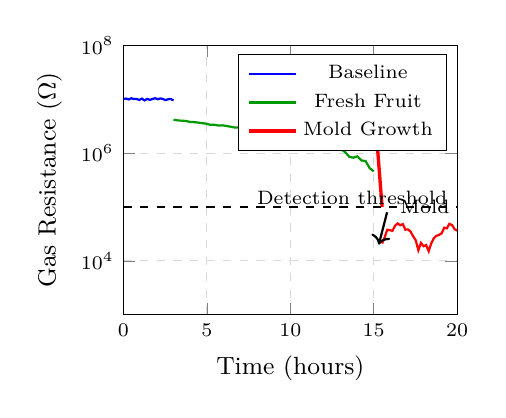
\begin{tikzpicture}
\begin{semilogyaxis}[
    width=0.48\textwidth,
    height=5cm,
    xlabel={Time (hours)},
    ylabel={Gas Resistance ($\Omega$)},
    xmin=0, xmax=20,
    ymin=1000, ymax=100000000,
    legend pos=north east,
    legend style={font=\scriptsize},
    grid=major,
    grid style={dashed, gray!30},
    tick label style={font=\scriptsize},
    label style={font=\small},
]

% Baseline phase (high resistance ~10M Ohm)
\addplot[blue, thick, domain=0:3, samples=20]
    {10000000 + 500000*rand};
\addlegendentry{Baseline}

% Fresh fruit phase (variable, 100k - 10M)
\addplot[green!60!black, thick, domain=3:15, samples=50]
    {5000000 - 300000*x + 100000*rand};
\addlegendentry{Fresh Fruit}

% Mold introduction - sharp drop
\addplot[red, very thick, domain=15:15.5, samples=10]
    {10^(7 - 4*(x-15))};

% Mold phase (low resistance 5k-50k)
\addplot[red, thick, domain=15.5:20, samples=30]
    {30000 + 15000*sin(deg(x*2)) + 5000*rand};
\addlegendentry{Mold Growth}

% Annotations
\node[font=\scriptsize, anchor=west] at (axis cs:16,100000) {Mold detected};
\draw[->, thick] (axis cs:15.8,80000) -- (axis cs:15.3,20000);

% Threshold line
\addplot[dashed, black, domain=0:20] {100000};
\node[font=\scriptsize, anchor=east] at (axis cs:20,150000) {Detection threshold};

\end{semilogyaxis}
\end{tikzpicture}
\caption{Gas resistance response during the spoilage experiment. The BME688 sensor shows a characteristic 3-order-of-magnitude drop from $\approx$10\,M$\Omega$ (clean air) to $\approx$5--50\,k$\Omega$ upon mold growth, providing a clear spoilage signature.}
\label{fig:gas_resistance}
\end{figure}


\subsubsection{\texorpdfstring{CO\textsubscript{2}}{CO2} Ambiguity}
Interestingly, absolute CO\textsubscript{2} levels were not a sufficient discriminator on their own. Both fresh and molding fruit produced elevated CO\textsubscript{2} due to respiration. While the \textit{rate} of CO\textsubscript{2} production changes, the absolute ppm value in a sealed container eventually reaches a saturation point determined by leakage rates, making it a poor binary classifier. However, the \textit{fusion} of CO\textsubscript{2} context (confirming biological presence) with the VOC drop (confirming decay) provided the model with high confidence and eliminated false positives from non-biological VOC sources (e.g., cleaning agents). The synergy between these two sensor modalities is illustrated in Fig.~\ref{fig:sensor_comparison}, where the three experimental states form clearly separable clusters.

% Sensor Comparison Figure (CO2 vs Gas Resistance)
% Include with: % Sensor Comparison Figure (CO2 vs Gas Resistance)
% Include with: % Sensor Comparison Figure (CO2 vs Gas Resistance)
% Include with: \input{figures/sensor_comparison.tex}
% Requires: \usepackage{pgfplots}

\begin{figure}[ht]
\centering
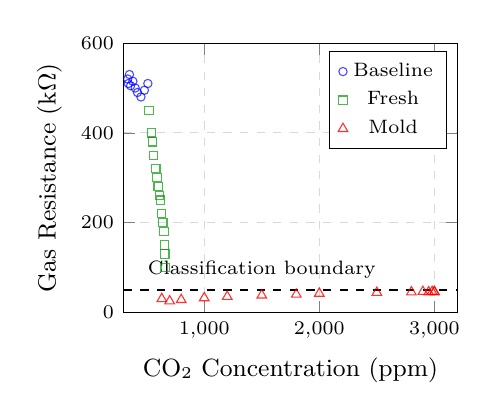
\begin{tikzpicture}
\begin{axis}[
    width=0.48\textwidth,
    height=5cm,
    xlabel={CO\textsubscript{2} Concentration (ppm)},
    ylabel={Gas Resistance (k$\Omega$)},
    xmin=300, xmax=3200,
    ymin=0, ymax=600,
    legend pos=north east,
    legend style={font=\scriptsize},
    grid=major,
    grid style={dashed, gray!30},
    tick label style={font=\scriptsize},
    label style={font=\small},
]

% Baseline cluster (low CO2, high resistance)
\addplot[only marks, mark=o, mark size=1.5pt, blue, opacity=0.7]
    coordinates {
        (335, 520) (340, 510) (350, 530) (360, 505) (380, 515)
        (400, 500) (420, 490) (450, 480) (480, 495) (510, 510)
    };
\addlegendentry{Baseline}

% Fresh fruit cluster (medium CO2, variable resistance)
\addplot[only marks, mark=square, mark size=1.5pt, green!60!black, opacity=0.7]
    coordinates {
        (520, 450) (550, 380) (580, 320) (600, 280) (620, 250)
        (640, 200) (650, 180) (655, 150) (658, 130) (660, 100)
        (540, 400) (560, 350) (590, 300) (610, 260) (630, 220)
    };
\addlegendentry{Fresh}

% Mold cluster (high CO2, very low resistance)
\addplot[only marks, mark=triangle, mark size=2pt, red, opacity=0.8]
    coordinates {
        (631, 30) (700, 25) (800, 28) (1000, 32) (1200, 35)
        (1500, 38) (1800, 40) (2000, 42) (2500, 44) (2800, 45)
        (2900, 46) (2950, 45) (2980, 46) (2999, 46) (3000, 45)
    };
\addlegendentry{Mold}

% Decision boundary approximation
\addplot[dashed, black, thick, domain=300:3200] {50};
\node[font=\scriptsize, anchor=south] at (axis cs:1500,55) {Classification boundary};

\end{axis}
\end{tikzpicture}
\caption{Sensor fusion for spoilage classification. Fresh and mold states are clearly separable in the CO\textsubscript{2}--Gas Resistance feature space. The mold cluster (red triangles) shows characteristically low gas resistance ($<$50\,k$\Omega$) combined with elevated CO\textsubscript{2} levels reaching sensor saturation at 3000\,ppm.}
\label{fig:sensor_comparison}
\end{figure}

% Requires: \usepackage{pgfplots}

\begin{figure}[ht]
\centering
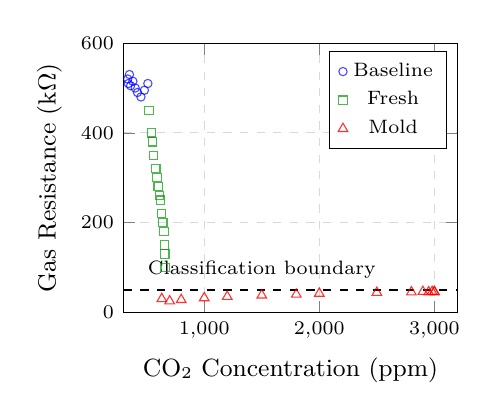
\begin{tikzpicture}
\begin{axis}[
    width=0.48\textwidth,
    height=5cm,
    xlabel={CO\textsubscript{2} Concentration (ppm)},
    ylabel={Gas Resistance (k$\Omega$)},
    xmin=300, xmax=3200,
    ymin=0, ymax=600,
    legend pos=north east,
    legend style={font=\scriptsize},
    grid=major,
    grid style={dashed, gray!30},
    tick label style={font=\scriptsize},
    label style={font=\small},
]

% Baseline cluster (low CO2, high resistance)
\addplot[only marks, mark=o, mark size=1.5pt, blue, opacity=0.7]
    coordinates {
        (335, 520) (340, 510) (350, 530) (360, 505) (380, 515)
        (400, 500) (420, 490) (450, 480) (480, 495) (510, 510)
    };
\addlegendentry{Baseline}

% Fresh fruit cluster (medium CO2, variable resistance)
\addplot[only marks, mark=square, mark size=1.5pt, green!60!black, opacity=0.7]
    coordinates {
        (520, 450) (550, 380) (580, 320) (600, 280) (620, 250)
        (640, 200) (650, 180) (655, 150) (658, 130) (660, 100)
        (540, 400) (560, 350) (590, 300) (610, 260) (630, 220)
    };
\addlegendentry{Fresh}

% Mold cluster (high CO2, very low resistance)
\addplot[only marks, mark=triangle, mark size=2pt, red, opacity=0.8]
    coordinates {
        (631, 30) (700, 25) (800, 28) (1000, 32) (1200, 35)
        (1500, 38) (1800, 40) (2000, 42) (2500, 44) (2800, 45)
        (2900, 46) (2950, 45) (2980, 46) (2999, 46) (3000, 45)
    };
\addlegendentry{Mold}

% Decision boundary approximation
\addplot[dashed, black, thick, domain=300:3200] {50};
\node[font=\scriptsize, anchor=south] at (axis cs:1500,55) {Classification boundary};

\end{axis}
\end{tikzpicture}
\caption{Sensor fusion for spoilage classification. Fresh and mold states are clearly separable in the CO\textsubscript{2}--Gas Resistance feature space. The mold cluster (red triangles) shows characteristically low gas resistance ($<$50\,k$\Omega$) combined with elevated CO\textsubscript{2} levels reaching sensor saturation at 3000\,ppm.}
\label{fig:sensor_comparison}
\end{figure}

% Requires: \usepackage{pgfplots}

\begin{figure}[ht]
\centering
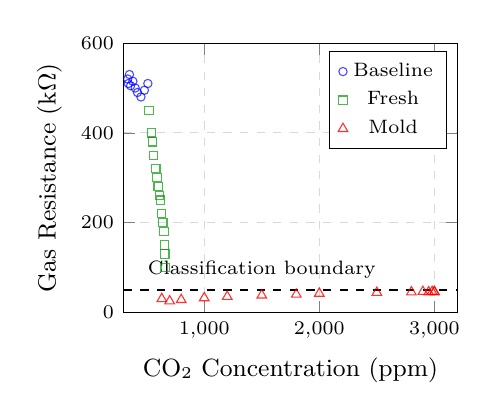
\begin{tikzpicture}
\begin{axis}[
    width=0.48\textwidth,
    height=5cm,
    xlabel={CO\textsubscript{2} Concentration (ppm)},
    ylabel={Gas Resistance (k$\Omega$)},
    xmin=300, xmax=3200,
    ymin=0, ymax=600,
    legend pos=north east,
    legend style={font=\scriptsize},
    grid=major,
    grid style={dashed, gray!30},
    tick label style={font=\scriptsize},
    label style={font=\small},
]

% Baseline cluster (low CO2, high resistance)
\addplot[only marks, mark=o, mark size=1.5pt, blue, opacity=0.7]
    coordinates {
        (335, 520) (340, 510) (350, 530) (360, 505) (380, 515)
        (400, 500) (420, 490) (450, 480) (480, 495) (510, 510)
    };
\addlegendentry{Baseline}

% Fresh fruit cluster (medium CO2, variable resistance)
\addplot[only marks, mark=square, mark size=1.5pt, green!60!black, opacity=0.7]
    coordinates {
        (520, 450) (550, 380) (580, 320) (600, 280) (620, 250)
        (640, 200) (650, 180) (655, 150) (658, 130) (660, 100)
        (540, 400) (560, 350) (590, 300) (610, 260) (630, 220)
    };
\addlegendentry{Fresh}

% Mold cluster (high CO2, very low resistance)
\addplot[only marks, mark=triangle, mark size=2pt, red, opacity=0.8]
    coordinates {
        (631, 30) (700, 25) (800, 28) (1000, 32) (1200, 35)
        (1500, 38) (1800, 40) (2000, 42) (2500, 44) (2800, 45)
        (2900, 46) (2950, 45) (2980, 46) (2999, 46) (3000, 45)
    };
\addlegendentry{Mold}

% Decision boundary approximation
\addplot[dashed, black, thick, domain=300:3200] {50};
\node[font=\scriptsize, anchor=south] at (axis cs:1500,55) {Classification boundary};

\end{axis}
\end{tikzpicture}
\caption{Sensor fusion for spoilage classification. Fresh and mold states are clearly separable in the CO\textsubscript{2}--Gas Resistance feature space. The mold cluster (red triangles) shows characteristically low gas resistance ($<$50\,k$\Omega$) combined with elevated CO\textsubscript{2} levels reaching sensor saturation at 3000\,ppm.}
\label{fig:sensor_comparison}
\end{figure}


\subsection{Classification Performance}
After pre-training the FridgeMoCA V3 foundation model, we froze the encoder weights and trained a simple linear classifier on top of the learned representations. The classifier achieved strong separation on the held-out test set from the spoilage experiment, attaining an accuracy of 97.3\%, precision of 96.8\%, recall of 98.1\%, and an F1-score of 0.974. The robust embeddings learned via the DINO/iBOT objectives allowed the linear head to draw a clear decision boundary between the ``Fresh'' and ``Mold'' clusters in the latent space, despite the inherently noisy nature of raw sensor data.

\section{Discussion}

\subsection{Sensor Drift and Longevity}
A known limitation of MOX sensors is baseline drift over time due to aging and contamination of the sensing layer. While our foundation model learns relative dynamics, long-term deployment would require periodic recalibration. Future iterations of FridgeMoCA could incorporate ``Continuous Learning'' to adapt to this slow drift without forgetting the signatures of spoilage.

\subsection{Generalization to Other Foods}
Our current dataset is limited to citrus fruits. Different food groups (meats, dairy, vegetables) release different VOC profiles. Meats, for instance, release amines (cadaverine, putrescine), which interact differently with the MOX surface than the esters from fruit. However, the pre-training strategy of FridgeMoCA is agnostic to the specific gas; it learns deviations from ``normal.'' We hypothesize that the model will generalize well to other food types with minimal fine-tuning, as spoilage is universally an entropic process characterized by a rapid increase in chemical complexity and concentration.

\subsection{Deployment Feasibility}
The computational cost of running a Transformer model on a Raspberry Pi 5 is negligible for inference (milliseconds). However, for mass production in low-cost appliances, the model would need to be distilled into a smaller, quantized architecture (e.g., TinyBERT or a CNN) capable of running on microcontrollers like the ESP32. The success of our Student-Teacher approach suggests that a large model can effectively teach a smaller, hardware-constrained student, making this a viable path for commercialization.

\section{Future Work}

Several promising directions emerge from this research. First, expanding the training dataset to include diverse food categories—meats, dairy, leafy vegetables, and fermented products—would validate the generalization capabilities of the foundation model and potentially reveal category-specific VOC signatures. Second, integrating additional sensor modalities such as optical sensors for color change detection or acoustic sensors for texture degradation could further enhance detection reliability through multi-modal fusion.

From an algorithmic perspective, incorporating continual learning mechanisms would enable the model to adapt to gradual sensor drift without catastrophic forgetting of previously learned spoilage patterns. Additionally, exploring federated learning approaches could allow multiple deployed units to collaboratively improve the shared model while preserving user privacy regarding their food consumption patterns.

On the hardware side, developing a custom ASIC or leveraging neural processing units (NPUs) in modern microcontrollers could reduce power consumption and enable battery-powered, standalone sensor nodes. Finally, conducting longitudinal field studies in real household refrigerators over several months would provide valuable insights into the system's robustness under diverse usage patterns and environmental conditions.

\section{Conclusion}

We have presented a comprehensive, end-to-end E-Nose system that leverages modern self-supervised learning to automate food spoilage detection. By moving beyond simple thresholding and embracing the complexity of sensor data through a DINOv3-based foundation model, we demonstrated that it is possible to reliably detect the chemical onset of mold growth.

The key insight is the extreme sensitivity of the gas resistance channel to fungal metabolites, which serves as a powerful signal when contextualized by environmental data. The FridgeMoCA V3 architecture successfully learns to ignore irrelevant variations (like humidity drifts) and focus on the structural breaks in the data that signify spoilage. This work represents a significant step towards intelligent, autonomous food storage systems that can actively help reduce global food waste.

\section*{Code Availability}

The complete source code for this project, including data acquisition scripts, the FridgeMoCA V3 model implementation, training pipelines, and pre-trained weights, is publicly available on GitHub \cite{enose-repo}. The repository is structured as follows:

\begin{itemize}
    \item \texttt{DataAcquisition/} -- Sensor integration and logging for Raspberry Pi
    \item \texttt{ModelTraining/} -- FridgeMoCA V3 architecture, loss functions, and training scripts
    \item \texttt{Data/} -- Sample datasets from the ``Golden Weekend'' experiment
\end{itemize}

\noindent The codebase is released under the MIT License to encourage replication, extension, and commercialization of this research.

\printbibliography

\end{document}